
% CVPR 2025 Paper Template; see https://github.com/cvpr-org/author-kit

\documentclass[10pt,twocolumn,letterpaper]{article}

%%%%%%%%% PAPER TYPE  - PLEASE UPDATE FOR FINAL VERSION
\usepackage{cvpr}              % To produce the CAMERA-READY version
% \usepackage[review]{cvpr}      % To produce the REVIEW version
\usepackage{cuted}
\usepackage{float}
\usepackage{algorithm}
\usepackage{algorithmic}
% \usepackage[pagenumbers]{cvpr} % To force page numbers, e.g. for an arXiv version
% Import additional packages in the preamble file, before hyperref
%
% --- inline annotations
%
\newcommand{\red}[1]{{\color{red}#1}}
\newcommand{\todo}[1]{{\color{red}#1}}
\newcommand{\TODO}[1]{\textbf{\color{red}[TODO: #1]}}
% --- disable by uncommenting  
% \renewcommand{\TODO}[1]{}
% \renewcommand{\todo}[1]{#1}

\usepackage{xcolor}
\usepackage{graphicx}
\usepackage{booktabs}
\usepackage{amsmath} 
\usepackage{amsfonts}
\usepackage{amssymb}
\usepackage{multirow} 
\usepackage{makecell}
\newcommand{\shline}{\Xhline{1.1pt}} % Adjust thickness as desired

% It is strongly recommended to use hyperref, especially for the review version.
% hyperref with option pagebackref eases the reviewers' job.
% Please disable hyperref *only* if you encounter grave issues, 
% e.g. with the file validation for the camera-ready version.
%
% If you comment hyperref and then uncomment it, you should delete *.aux before re-running LaTeX.
% (Or just hit 'q' on the first LaTeX run, let it finish, and you should be clear).
\definecolor{cvprblue}{rgb}{0.21,0.49,0.74}
\usepackage[pagebackref,breaklinks,colorlinks,allcolors=cvprblue]{hyperref}
\newcommand{\yijun}[1]{\textcolor{magenta}{[{\bf YJ--} #1]}}
\newcommand{\yc}[1]{\textcolor{blue}{[{\bf yc--} #1]}}
%%%%%%%%% PAPER ID  - PLEASE UPDATE
\def\paperID{4797} % *** Enter the Paper ID here
\def\confName{CVPR}
\def\confYear{2025}

%%%%%%%%% TITLE - PLEASE UPDATE
\title{TransPixar: Advancing Text-to-Video Generation with Transparency}


%%%%%%%%% AUTHORS - PLEASE UPDATE
\author{
Luozhou Wang\textsuperscript{$1$}\thanks{This work was done during an internship at Adobe Research.} \quad
Yijun Li\textsuperscript{$3$}\thanks{Project Leader}\quad
Zhifei Chen\textsuperscript{$1$} \quad
Jui-Hsien Wang\textsuperscript{$3$} \quad
Zhifei Zhang\textsuperscript{$3$} \quad
He Zhang\textsuperscript{$3$} \quad \\
Zhe Lin\textsuperscript{$3$} \quad
Yingcong Chen\textsuperscript{$1,2$}\thanks{Corresponding author} \quad
\\
$^1$ HKUST(GZ).\quad 
$^2$ HKUST.\quad 
$^3$ Adobe Research.
}


\begin{document}
\maketitle
\begin{strip}
    \centering
    \vspace{-5em}
    \centering
    \includegraphics[width=\textwidth]{figs/teaser.pdf}
    \vspace{-2em}
    \captionof{figure}{\textbf{RGBA Video Generation with TransPixar.} By introducing LoRA layers into DiT-based text-to-video model with a novel alpha channel adaptive attention mechanism, our method enables RGBA video generation from text while preserving Text-to-Video quality. 
    }
    \label{fig:teaser}
\end{strip}

\begin{abstract}
Segment Anything Model 2 (SAM 2) has emerged as a powerful tool for video object segmentation and tracking anything. Key components of SAM 2 that drive the impressive video object segmentation performance include a large multistage image encoder for frame feature extraction and a memory mechanism that stores memory contexts from past frames to help current frame segmentation. The high computation complexity of multistage image encoder and memory module has limited its applications in real-world tasks, e.g., video object segmentation on mobile devices. To address this limitation, we propose EfficientTAMs, lightweight track anything models that produce high-quality results with low latency and model size. Our idea is based on revisiting the plain, nonhierarchical Vision Transformer (ViT) as an image encoder for video object segmentation, and introducing an efficient memory module, which reduces the complexity for both frame feature extraction and memory computation for current frame segmentation. We take vanilla lightweight ViTs and efficient memory module to build EfficientTAMs, and train the models on SA-1B and SA-V datasets for video object segmentation and track anything tasks. We evaluate on multiple video segmentation benchmarks including semi-supervised VOS and promptable video segmentation, and find that our proposed EfficientTAM with vanilla ViT perform comparably to SAM 2 model (HieraB+SAM 2) with $\sim$2x speedup on A100 and $\sim$2.4x  parameter reduction. On segment anything image tasks, our EfficientTAMs also perform favorably over original SAM with $\sim$20x  speedup on A100 and $\sim$20x  parameter reduction. On mobile devices such as iPhone 15 Pro Max, our EfficientTAMs can run at $\sim$10 FPS for performing video object segmentation with reasonable quality, highlighting the capability of small models for on-device video object segmentation applications. 
\end{abstract}    
\section{Introduction}
Deep learning techniques have made rapid progress in conditional image generation. For example, networks have been used to inpaint missing image regions~\citep{pathakCVPR16context,yang2016high,isola2016image}, 
add color to grayscale images~\citep{iizuka2016let,larsson2016learning,zhang2016colorful,isola2016image}, and generate photorealistic images from sketches~\cite{sangkloy2017scribbler,isola2016image}.
However, most techniques in this space have focused on generating a \textit{single} result.
In this work, we model a \textit{distribution} of potential results, as many of these problems may be multimodal in nature. For example,
as seen in Figure~\ref{fig:teaser}, an image captured at night may look very different in the day, depending on cloud patterns and lighting conditions.
We pursue two main goals: producing results which are (1) perceptually realistic and (2) diverse, all while remaining faithful to the input.

Mapping from a high-dimensional input to a high-dimensional output distribution is challenging. A common approach to representing multimodality is learning a low-dimensional latent code, which should represent aspects of the possible outputs not contained in the input image. At inference time, a deterministic generator uses the input image, along with stochastically sampled latent codes, to produce randomly sampled outputs. A common problem in existing methods is~\textit{mode collapse}~\citep{goodfellow2016nips}, where only a small number of real samples get represented in the output.
We systematically study a family of solutions to this problem.

We start with the \pp framework~\citep{isola2016image}, which has previously been shown to produce high-quality results for various image-to-image translation tasks. The method trains a generator network, conditioned on the input image, with two losses: (1) a regression loss to produce similar output to the known paired ground truth image and (2) a learned discriminator loss to encourage realism. The authors note that trivially appending a randomly drawn latent code did not produce diverse results. Instead, we propose encouraging a bijection between the output and latent space. 
We not only perform the direct task of mapping the latent code (along with the input) to the output but also jointly learn an encoder from the output back to the latent space. 
This discourages two different latent codes from generating the same output (non-injective mapping).
During training, the learned encoder attempts to pass enough information to the generator to resolve any ambiguities regarding the output mode.
For example, when generating a day image from a night image, the latent vector may encode information about the sky color, lighting effects on the ground, and cloud patterns.  Composing the encoder and generator sequentially should result in the same image being recovered. The opposite should produce the same latent code.

\begin{figure}
\centering
\includegraphics[width=1.\linewidth]{imgs/teaser.pdf}
\vspace{-4mm}
\caption{\small Multimodal image-to-image translation using our proposed method: given an input image from one domain (night image of a scene), we aim to model a \textit{distribution} of potential outputs in the target domain (corresponding day images), producing both realistic and diverse results.}
\vspace{-4mm}
\label{fig:teaser}
\end{figure}


In this work, we instantiate this idea by exploring several objective functions, inspired by literature in unconditional generative modeling:
  \begin{itemize}[leftmargin=0.1in]
  
    \item \textbf{\cvaegan (Conditional Variational Autoencoder GAN)}:
    One approach is first encoding the ground truth image into the latent space, giving the generator a noisy ``peek" into the desired output. Using this, along with the input image, the generator should be able to reconstruct the specific output image. To ensure that random sampling can be used during inference time, the latent distribution is regularized using KL-divergence to be close to a standard normal distribution. This approach has been popularized in the unconditional setting by VAEs~\citep{kingma2013auto} and VAE-GANs~\citep{larsen2016vaegan}.
    
    \item \textbf{\cinfogan (Conditional Latent Regressor GAN)}: Another approach is to first provide a randomly drawn latent vector to the generator. In this case, the produced output may not necessarily look like the ground truth image, but it should look realistic. An encoder then attempts to recover the latent vector from the output image. This method could be seen as a conditional formulation of the ``latent regressor" model~\citep{donahue2016adversarial,dumoulin2016adversarially} and also related to InfoGAN~\citep{xi2016infogan}.
    
    \item \textbf{\bicycle}: Finally, we combine both these approaches to enforce the connection between latent encoding and output in both directions {\em jointly} and achieve improved performance. We show that our method can produce both diverse and visually appealing results across a wide range of image-to-image translation problems, significantly more diverse than other baselines, including naively adding noise in the \pp framework. In addition to the loss function, we study the performance with respect to several encoder networks, as well as different ways of injecting the latent code into the generator network. 
\end{itemize}

We perform a systematic evaluation of these variants by using humans to judge photorealism and a perceptual distance metric~\cite{zhang2018unreasonable} to assess output diversity. Code and data are available at \url{https://github.com/junyanz/BicycleGAN}.
\section{Related Work}
\label{sec:related_work}
We briefly review prior works on fast and efficient neural networks and differentiate this work from them.

\medskip\noindent\textbf{CNN.} \enspace
CNNs are the mainstream architecture in the computer vision field, especially when it comes to deployment in practice, where being fast is as important as being accurate. Though there have been numerous studies~\cite{sifre2014rigid,singh2019hetconv,chen2019drop,chollet2017xception,zhang2017interleaved,li2021micronet,he2022tackling,zhuo2022semi} to achieve higher efficiency, the rationale behind them is more or less to perform a low-rank approximation. Specifically, the group convolution~\cite{krizhevsky2012imagenet} and the depthwise separable convolution~\cite{sifre2014rigid} (consisting of depthwise and pointwise convolutions) are probably the most popular ones. They have been widely adopted in mobile/edge-oriented networks, such as MobileNets~\cite{howard2017mobilenets,sandler2018mobilenetv2,howard2019searching},
ShuffleNets~\cite{zhang2018shufflenet,ma2018shufflenet}, GhostNet~\cite{han2020ghostnet},
EfficientNets~\cite{tan2019efficientnet,tan2021efficientnetv2}, TinyNet~\cite{han2020model}, Xception~\cite{chollet2017xception}, CondenseNet~\cite{huang2018condensenet,yang2021condensenet}, TVConv~\cite{chen2022tvconv}, MnasNet\cite{tan2019mnasnet}, and FBNet~\cite{wu2019fbnet}. While they exploit the redundancy in filters to reduce the number of parameters and FLOPs, they suffer from increased memory access when increasing the network width to compensate for the accuracy drop. By contrast, we consider the redundancy in feature maps and propose a partial convolution to reduce FLOPs and memory access \emph{simultaneously}. 

\medskip\noindent\textbf{ViT, MLP, and variants.} \enspace
 There is a growing interest in studying ViT ever since Dosovitskiy \etal~\cite{dosovitskiy2020image} expanded the application scope of transformers~\cite{vaswani2017attention} from machine translation~\cite{vaswani2017attention} or forecasting~\cite{wen2022social} to the computer vision field. Many follow-up works have attempted to improve ViT in terms of training setting~\cite{touvron2021training,touvron2022deit,steiner2021train} and model design~\cite{liu2021swin,liu2022swin,wang2021pyramid,graham2021levit,zhong2022tree}. One notable trend is to pursue a better accuracy-latency trade-off by reducing the complexity of the attention operator~\cite{ali2021xcit,vaswani2021scaling,huang2022lightvit,lu2021soft,tang2022quadtree}, incorporating convolution into ViTs~\cite{dai2021coatnet,chen2022mobile,srinivas2021bottleneck}, or doing both~\cite{cai2022efficientvit,li2022efficientformer,pan2022edgevits,mehta2022separable}. Besides, other studies~\cite{tolstikhin2021mlp,lian2021mlp,chen2021cyclemlp} propose to replace the attention with simple MLP-based operators. However, they often evolve to be CNN-like~\cite{liu2022we}. In this paper, we focus on analyzing the convolution operations, particularly DWConv, due to the following reasons: First, the advantage of attention over convolution is unclear or debatable~\cite{wang2022shift,liu2022convnet}. Second, the attention-based mechanism generally runs slower than its convolutional counterparts and thus  becomes less favorable for the current industry~\cite{mehta2021mobilevit,hu2019local}. Finally, DWConv is still a popular choice in many hybrid models, so it is worth a careful examination.
 
\section{Method}
\label{sec:method}

\begin{figure*}[t]
    \centering
    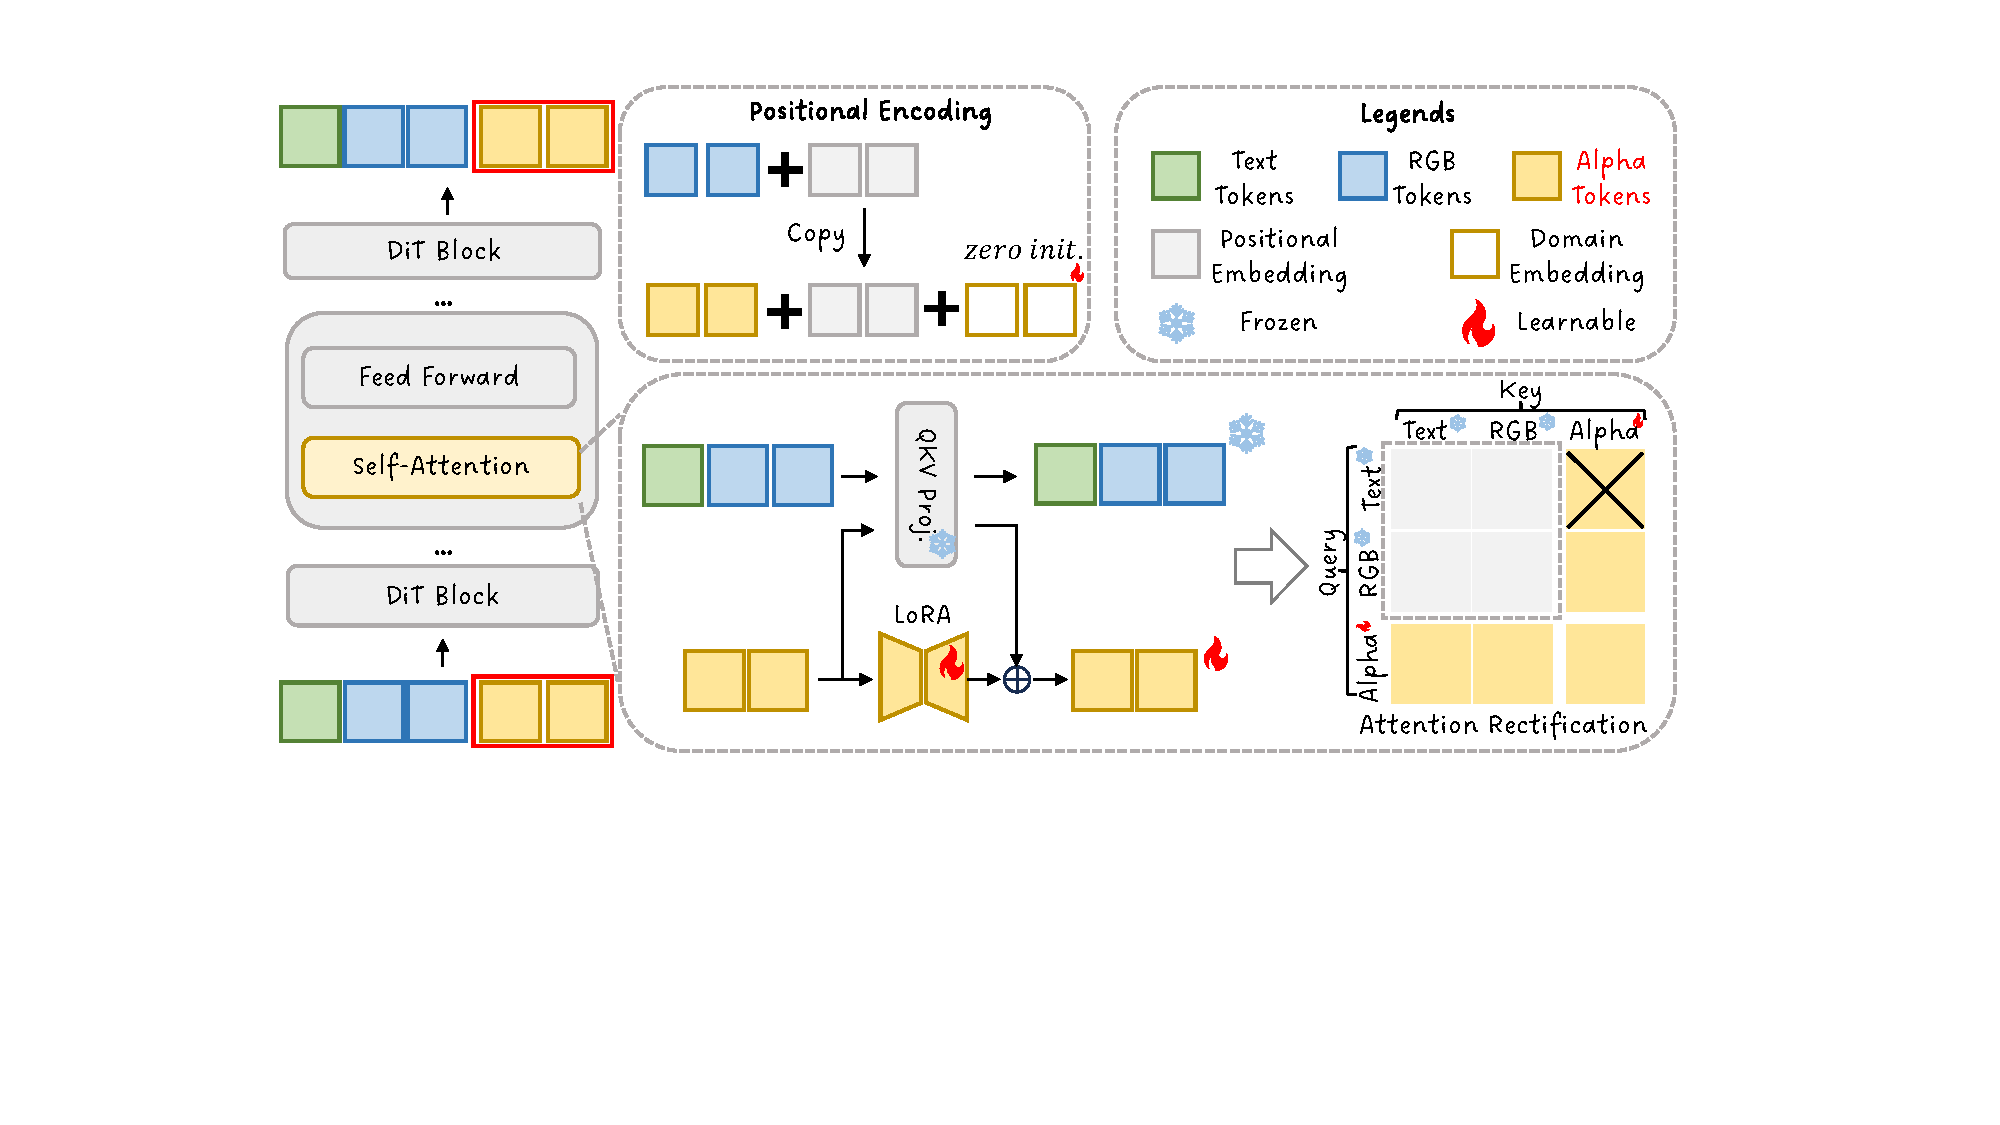
\includegraphics[width=1.0\linewidth]{figs/method-pipeline.pdf}
    \vspace{-0.2in}
    \caption{\textbf{Pipeline of TransPixar.} Our method is organized as follows: (1) \textbf{Left}: we extend the input of DiT to include new alpha tokens; (2) \textbf{Top Center}: we initialize alpha tokens with our positional encoding; (3) \textbf{Bottom Cente}r: we insert a partial LoRA and adjust attention computation during training and inference.}
    \label{fig-pipeline}
    \vspace{-0.1in}
\end{figure*}


% %-------------------------------------------------------------------------
\subsection{Preliminary}
We first introduce the open-sourced state-of-the-art DiT-based video generation models~\cite{yang2024cogvideox,genmo2024mochi}.
The core components of DiT-based video models are attention modules, and there are two primary distinctions between these models and previous approaches.
On one hand, unlike previous models that alternate between 1D temporal attention and 2D spatial attention~\cite{cerspense2023zeroscope, chen2023videocrafter1, chen2024videocrafter2, opensora}, current methods typically employ 3D spatio-temporal attention, allowing them to capture spatio-temporal dependencies more effectively.
On the other hand, instead of using cross-attention for text conditioning, these models concatenate text tokens \( \mathbf{x}_{\text{text}} \) with visual tokens \( \mathbf{x}_{\text{video}} \) into a single long sequence. 
The shape of video tokens and text tokens are \(B\times L\times D\) and \(B\times L_{\text{text}}\times D\), wher \(B\) equals to batch size, \(L_{\text{text}}\) equals to the length of text tokens, \(L\) equals to the length of video tokens and \(D\) equals to the latent dimension of transformer.
Full self-attention is then applied across the combined sequence:
\begin{equation}
\begin{aligned}
    &\text{Attention}(\mathbf{Q}, \mathbf{K}, \mathbf{V}) = \text{softmax}\left(\frac{\mathbf{Q}\mathbf{K}^T}{\sqrt{d_k}}\right)\mathbf{V}, \quad \text{where} \\
&\mathbf{Z : Z \in \{Q, K, V\}} \\&= [\mathbf{W}_{z : z \in \{q, k, v\}}(\mathbf{x}_{\text{text}}); \mathbf{f}_{z : z \in \{q, k, v\}}(\mathbf{x}_{\text{video}})]
\end{aligned}
\label{SA}
\end{equation}


Here \( \mathbf{W}_{t} \) (for \( t \in \{q, k, v\} \)) represents the projection matrixs in the transformer model, and \( \mathbf{f}_{t} \) (for \( t \in \{q, k, v\} \)) represents a combined operation that incorporates both the projection and positional encoding for visual tokens. 
There are two commonly used types of positional encoding. One is absolute positional encoding formulated as follows:
\begin{equation}
\begin{aligned}
\mathbf{f}_{z : z \in \{q, k, v\}}(\mathbf{x}_{\text{video}}) := \mathbf{W}_{z : z \in \{q, k, v\}}(\mathbf{x}_{\text{video}}^m + \mathbf{p}^m),
\end{aligned}
\label{PE}
\end{equation}
where \( \mathbf{p} \) is the positional embedding (e.g., a sinusoidal function) and \( m \) denotes the position of each RGB video token.
Another approach is the Rotary Position Embedding (RoPE)~\cite{su2024roformer}, often used by~\cite{yang2024cogvideox, genmo2024mochi}. 
This is expressed as
\begin{equation}
\begin{aligned}
\mathbf{f}_{z : z \in \{q, k\}}(\mathbf{x}_{\text{video}}) := \mathbf{W}_{z : z \in \{q, k\}}(\mathbf{x}_{\text{video}}^m) \circ e^{im\theta},
\end{aligned}
\label{RoPE}
\end{equation}
where \( m \) is the positional index, \( i \) is the imaginary unit for rotation, and \( \theta \) is the rotation angle.




% %-------------------------------------------------------------------------
\subsection{Our Approach} 
To jointly generate RGB and alpha videos, we adapt a pretrained RGB video generation model through several modifications. The whole pipeline is visualized in Fig.~\ref{fig-pipeline}.

Firstly, we double the sequence length of noisy input tokens to enable the model to generate videos of double length, from \( \mathbf{x}^{1:L}_{\text{video}} \) to \( \mathbf{x}^{1:2*L}_{\text{video}} \). 
Here, \( \mathbf{x}^{1:L}_{\text{video}} \) will be decoded into the RGB video, while \( \mathbf{x}^{L+1:2*L}_{\text{video}} \) will be decoded into the corresponding alpha video.
The Query(Q), Key(K), Value(V) representations are formulated as:
\begin{equation}
\begin{aligned}
&\mathbf{Z : Z \in \{Q, K, V\}} \\&= [\mathbf{W}_{z : z \in \{q, k, v\}}(\mathbf{x}_{\text{text}}); \mathbf{f}_{z : z \in \{q, k, v\}}(\mathbf{x}^{1:2*L}_{\text{video}})]
\end{aligned}
\end{equation}

In addition to sequence doubling, we explored increasing batch size or latent dimensions and splitting output into two domains; however, these approaches showed limited effectiveness under constrained datasets, which we discuss later.

Secondly, we modify the positional encoding function \( \mathbf{f}_{t : t \in \{q, k, v\}}(\cdot) \), as shown in Fig.~\ref{fig-pe}.
Instead of continuously numbering indices, we allow RGB and alpha tokens to share the same positional encoding. 
Taking absolute positional encoding as an example:
\begin{equation}
\begin{aligned}
&\mathbf{f}^*_{z : z \in \{q, k, v\}}(\mathbf{x}_{\text{video}}) \\:=
&\begin{cases}
\mathbf{W}_{z : z \in \{q, k, v\}}(\mathbf{x}_{\text{video}}^m + \mathbf{p}^m), & \text{if } m \leq L, \\
\mathbf{W}^*_{z : z \in \{q, k, v\}}(\mathbf{x}_{\text{video}}^m + \mathbf{p}^{m-L} + d), & \text{if } m > L.
\end{cases}
\label{eq:our_pe}
\end{aligned}
\end{equation}

Here we introduce a domain embedding \( d \), initialized to zero. We make it learnable to help the model adaptively differentiate between RGB (\(m\leq L\)) and alpha tokens (\(m>L \)). 
%
The motivation behind this design is we observe that with same postional encoding, even initializing with different noises, the tokens from two domains tend to generate same results. 
It minimizes spatial-temporal alignment challenges at the very beginning of training and thus accelerates convergence.

Next we propose a fine-tuning scheme using LoRA~\cite{hu2021lora}, in which the LoRA layer is applied only to alpha domain tokens:
\begin{equation}
\begin{aligned}
&\mathbf{W}^*_{z : z \in \{q, k, v\}}(\mathbf{x}_{\text{video}}^m + \mathbf{p}^{m-L} + d)\\=
&\ \mathbf{W}_{z : z \in \{q, k, v\}}(\mathbf{x}_{\text{video}}^m + \mathbf{p}^{m-L} + d)
\\
+\ &\gamma\cdot \text{LoRA}(\mathbf{x}_{\text{video}}^m + \mathbf{p}^{m-L} + d), \quad \text{if } m > L,
\label{eq:our_lora}
\end{aligned}
\end{equation}
where \( \gamma \) controls the residual strength. 
Additionally, we design an attention mask to block unwanted attention computation. 
Given a text-video token sequence length \( L_\text{text} + 2L \), where \( L_\text{text} \) represents text token length, the mask is defined as:
\begin{equation}
\mathbf{M}^*_{mn} = 
\begin{cases} 
-\infty, & \text{if } m \leq L_\text{text} \ \text{and} \ \, n > L_\text{text} + L, \\
0, & \text{otherwise}.
\end{cases}
\label{eq:attn_mask}
\end{equation}

Combining these modifications, inference with our method is expressed as:
\begin{equation}
\begin{aligned}
    &\text{Attention}(\mathbf{Q}, \mathbf{K}, \mathbf{V}) = \text{softmax}\left(\frac{\mathbf{Q}\mathbf{K}^T}{\sqrt{d_k}}+\mathbf{M}^*\right)\mathbf{V}, \quad \text{where} \\
&\mathbf{Z : Z \in \{Q, K, V\}} \\&= [\mathbf{W}_{z : z \in \{q, k, v\}}(\mathbf{x}_{\text{text}}); \mathbf{f}^*_{z : z \in \{q, k, v\}}(\mathbf{x}_{\text{video}})]
\end{aligned}
\label{eq:our_method}
\end{equation}

Training is carried out using flow matching~\cite{liu2022flow} or a traditional diffusion process~\cite{ho2020denoising}.


\begin{figure}[t]
    \centering
    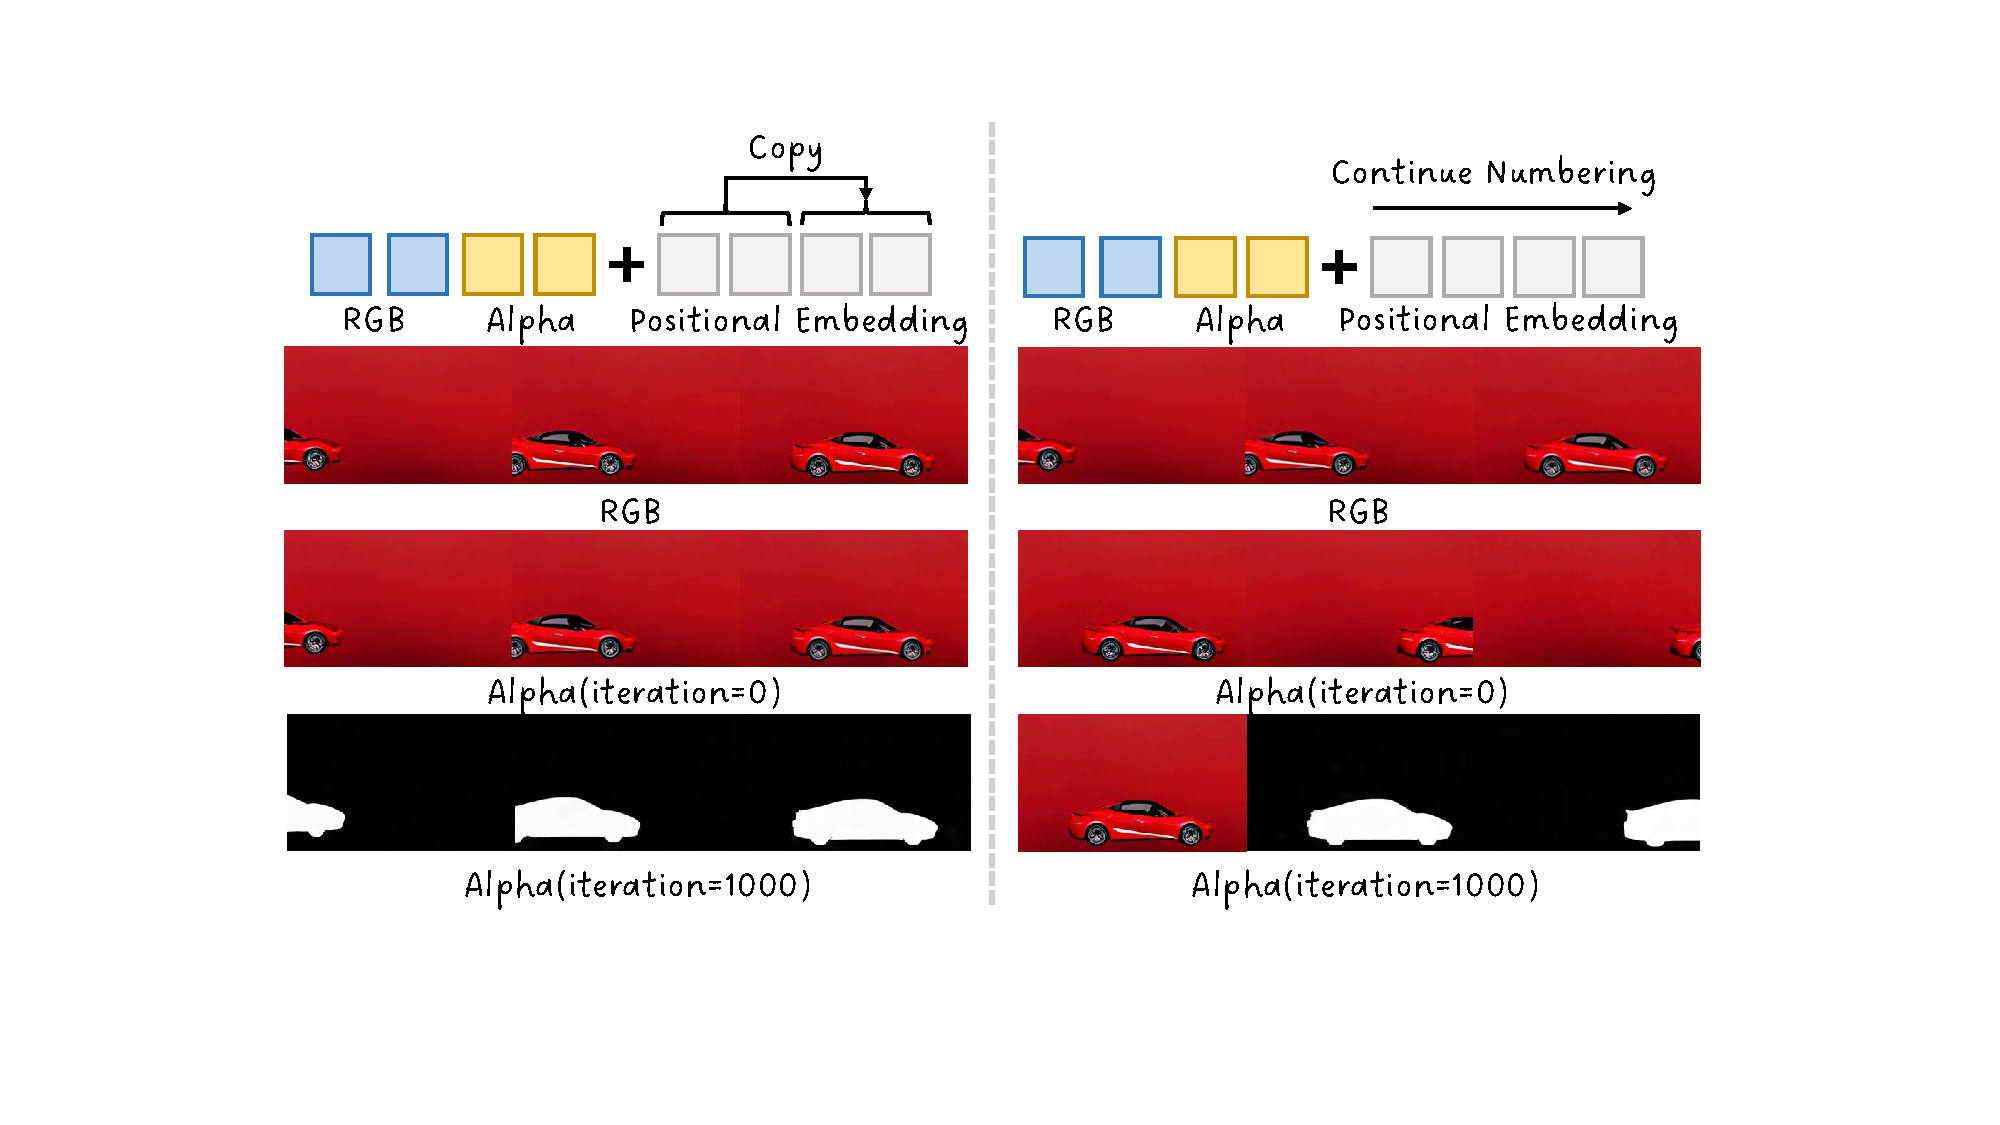
\includegraphics[width=1.0\linewidth]{figs/method-pe_init.pdf}
    \vspace{-0.2in}
    \caption{\textbf{Positional Encoding Design for RGBA Generation.} Assigning alpha tokens the same positional encoding as RGB yields similar results, resulting in faster convergence after 1000 iterations compared to standard encoding strategies.}
    \label{fig-pe}
    \vspace{-0.1in}
\end{figure}

% %-------------------------------------------------------------------------
\subsection{Analysis}
% % given our goal is 最大程度地继承 pretrain video model的能力,让它能生成的东西超越已有的RGBA训练集,
% 在目前我们使用的3d full attention DiT的video generation model的框架下,最重要的计算是attention mechanism,因此我们进一步对该过程进行分析:
% The attention matrix, \(\mathbf{Q}\mathbf{K}^T\), now has dimensions \((L_\text{text} + 2*L) \times (L_\text{text} + 2*L)\), which we simplify by organizing it into a 3x3 grouped attention matrix—\textbf{Text-attend-to-RGB}, \textbf{RGB-attend-to-Text}, and so forth, as illustrated in Fig.~\ref{fig-pipeline}. Then we procceed to analyze them:

% \noindent{\textbf{Text-Attend-to-RGB} and \textbf{RGB-Attend-to-Text}}.
% Given this matrix, we are supposed to preserve as much of the computation in the upper-left 2x2 section as possible so that we can preserve the RGB generation potential. 

% These represent the upper-left 2x2 section in \(\mathbf{Q}\mathbf{K}^T\) and 是RGB original generation model有且仅有的计算过程,如果我们能保证这部分计算不受影响,we can replicate the original RGB generation performance. 
% Therefore, we limited the scope of LoRA's influence, as defined in Equation~\eqref{eq:our_lora}, we retain the original QKV values for both text and RGB tokens, maintaining the pretrained model’s behavior in these domains.

% Besides the partial lora, the introduction of alpha tokens make the text and RGB tokens need to act as key and interact with alpha tokens as query, which will also 改变这个2x2 attention matrix的计算结果。
% Therefore, we proceed to analyze two additional attention computations that affect RGB generation shown in Fig.~\ref{fig-attn}:


% \noindent{\textbf{Text-Attend-to-Alpha}}: We find this attention is detrimental to the generation quality. 
% Since the model is originally trained with text and RGB data, introducing attention from text to alpha causes interference due to the domain gap between alpha and RGB. 
% Specifically, alpha modality provide only contour information and lack the rich texture, color, and semantic details associated with text prompt, thereby degrading generation quality. 
% To mitigate this, we design the attention mask (Equation~\eqref{eq:attn_mask}) that blocks this computation.

% \noindent{\textbf{RGB-Attend-to-Alpha}}: In contrast, we identify \textbf{RGB-to-Alpha} as essential for successful joint generation. 
% This attention allows the model to refine RGB tokens by considering alpha information, facilitating alignment between generated RGB and alpha channels. 
% This refinement process is a critical component missing in prior generation-then-prediction pipelines, which lack a feedback mechanism for RGB refinement based on alpha guidance.
Given our goal of maximizing the inherited capabilities of the pretrained video model, enabling it to generate beyond the existing RGBA training set, we analyze the most critical component within our current 3D full attention DiT video generation model: the attention mechanism.
%
The attention matrix, \(\mathbf{Q}\mathbf{K}^T\), has dimensions \((L_\text{text} + 2*L) \times (L_\text{text} + 2*L)\), which we simplify by organizing it into a 3x3 grouped attention matrix—including \textbf{Text-attend-to-RGB}, \textbf{RGB-attend-to-Text}, and so forth, as illustrated in Fig.~\ref{fig-pipeline}. %We then analyze these components:

\vspace{0.5em}
\noindent\textbf{Text-Attend-to-RGB and RGB-Attend-to-Text}. These represent the upper-left 2x2 section of  and are computations that exist solely in the original RGB generation model. If we ensure that this part of the computation remains unaffected, we can replicate the original RGB generation performance. Therefore, we limit the scope of LoRA's influence, as defined in Eq.~\eqref{eq:attn_mask}, by retaining the original QKV values for both text and RGB tokens, thus preserving the pretrained model’s behavior in these domains.

Besides the partial LoRA, the added alpha tokens requires the text and RGB tokens to also act as queries and interact with the alpha tokens as keys, which alters the computation in this 2x2 attention matrix. 
Therefore, we further analyze two additional attention computations that impact RGB generation, as shown in Fig.~\ref{fig-attn}.

\vspace{0.5em}
\noindent\textbf{Text-Attend-to-Alpha.} We find that this attention is detrimental to the generation quality. Since the model was originally trained with text and RGB data, introducing attention from text to alpha causes interference due to the domain gap between alpha and RGB. Specifically, the alpha modality provides only contour information and lacks the rich texture, color, and semantic details associated with the text prompt, thereby degrading generation quality. To mitigate this, we design the attention mask (Eq.~\eqref{eq:attn_mask}) that blocks this computation.

\vspace{0.5em}
\noindent\textbf{RGB-Attend-to-Alpha.} In contrast, we identify \textbf{RGB-to-Alpha} as essential for successful joint generation. This attention allows the model to refine RGB tokens by considering alpha information, facilitating alignment between generated RGB and alpha channels. This refinement process is a critical component missing in previous generation-then-prediction pipelines, which lacked a feedback mechanism for RGB refinement based on alpha guidance.


\begin{figure}[t]
    \centering
    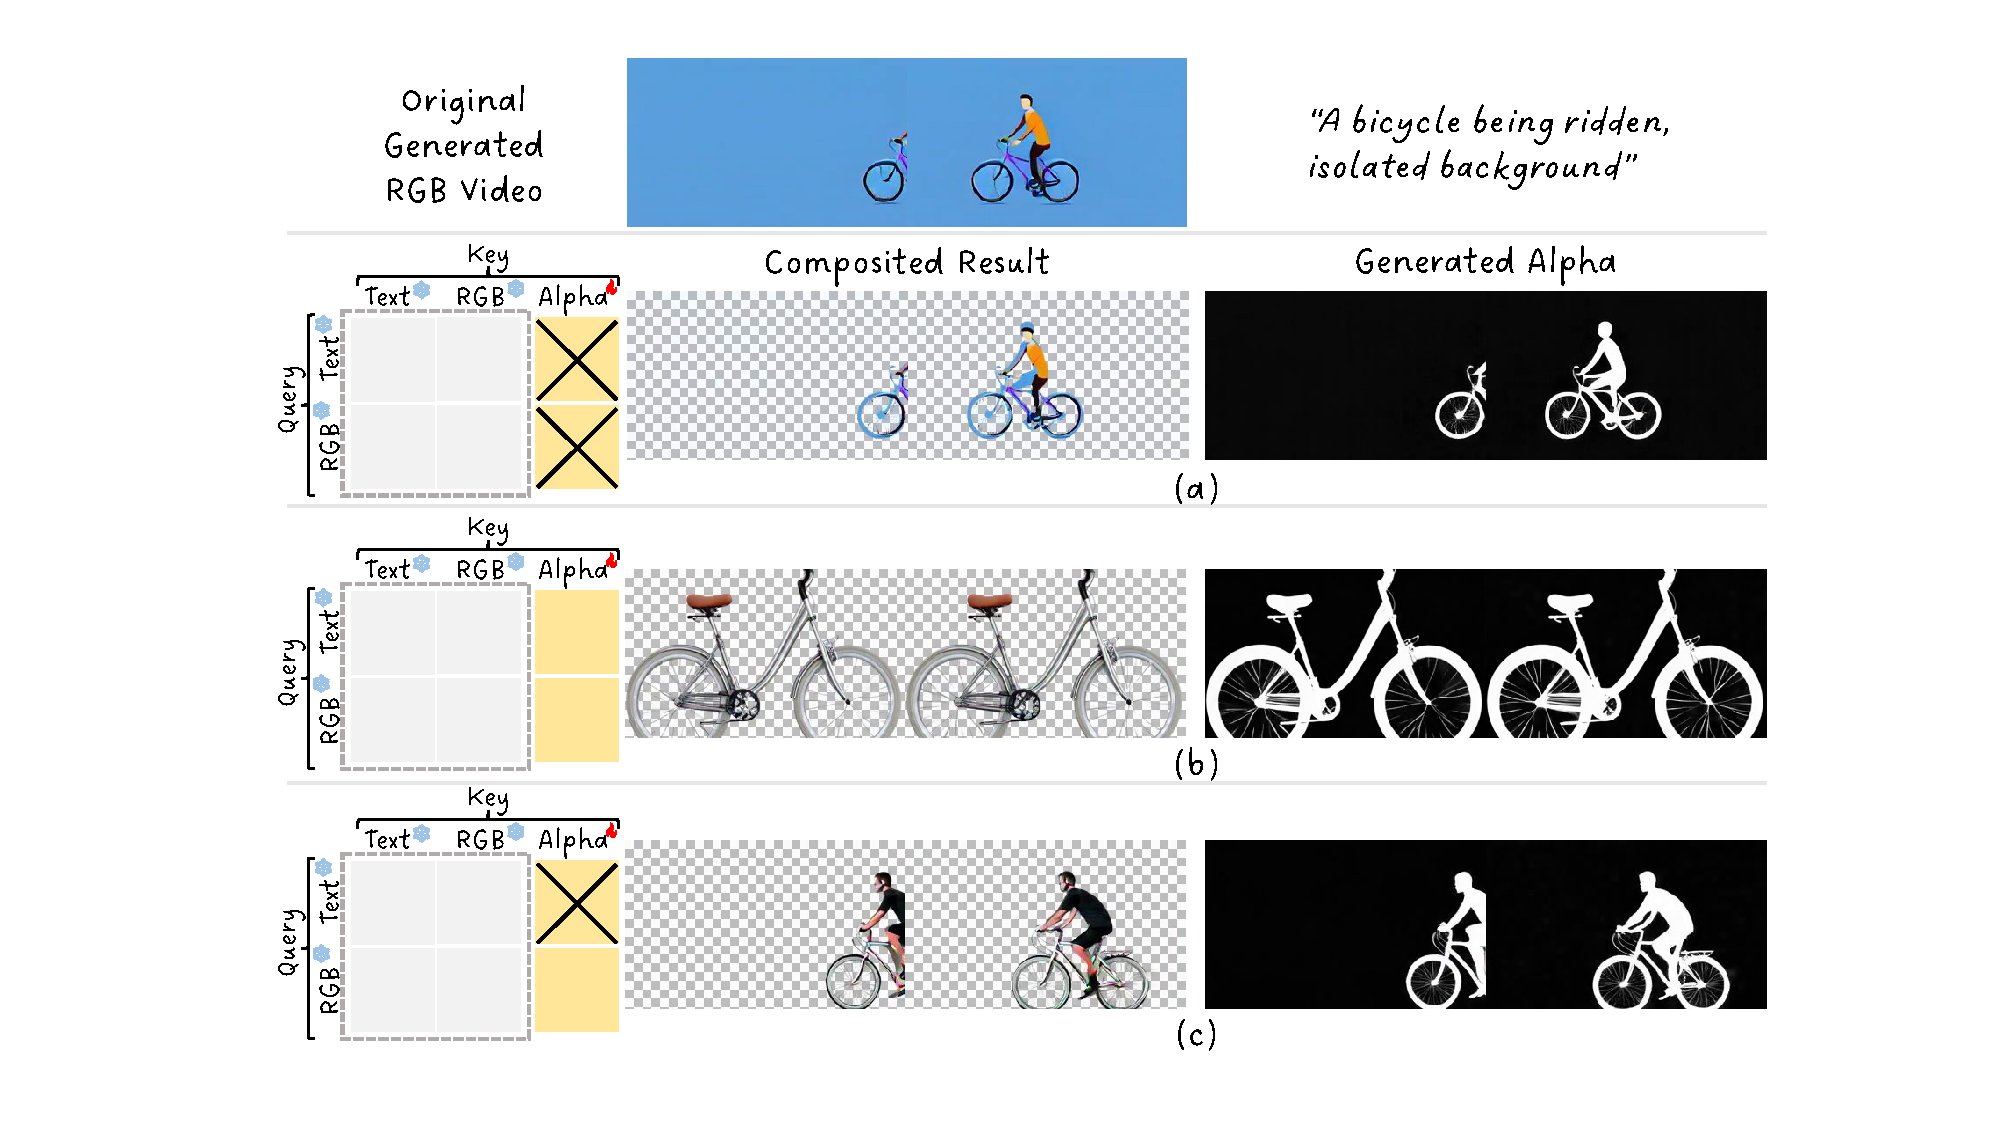
\includegraphics[width=1.0\linewidth]{figs/method-attn.pdf}
    \vspace{-0.2in}
    \caption{\textbf{Attention Rectification.} (a) Eliminating all attention from alpha as a key preserves 100\% RGB generation but leads to poor alignment. (b) Retaining all attention significantly degrades quality, causing a lack of motion in bicycles. (c) Our method achieves an effective balance.
    }
    \label{fig-attn}
    \vspace{-0.1in}
\end{figure}




\begin{figure*}[htbp]
    \centering
    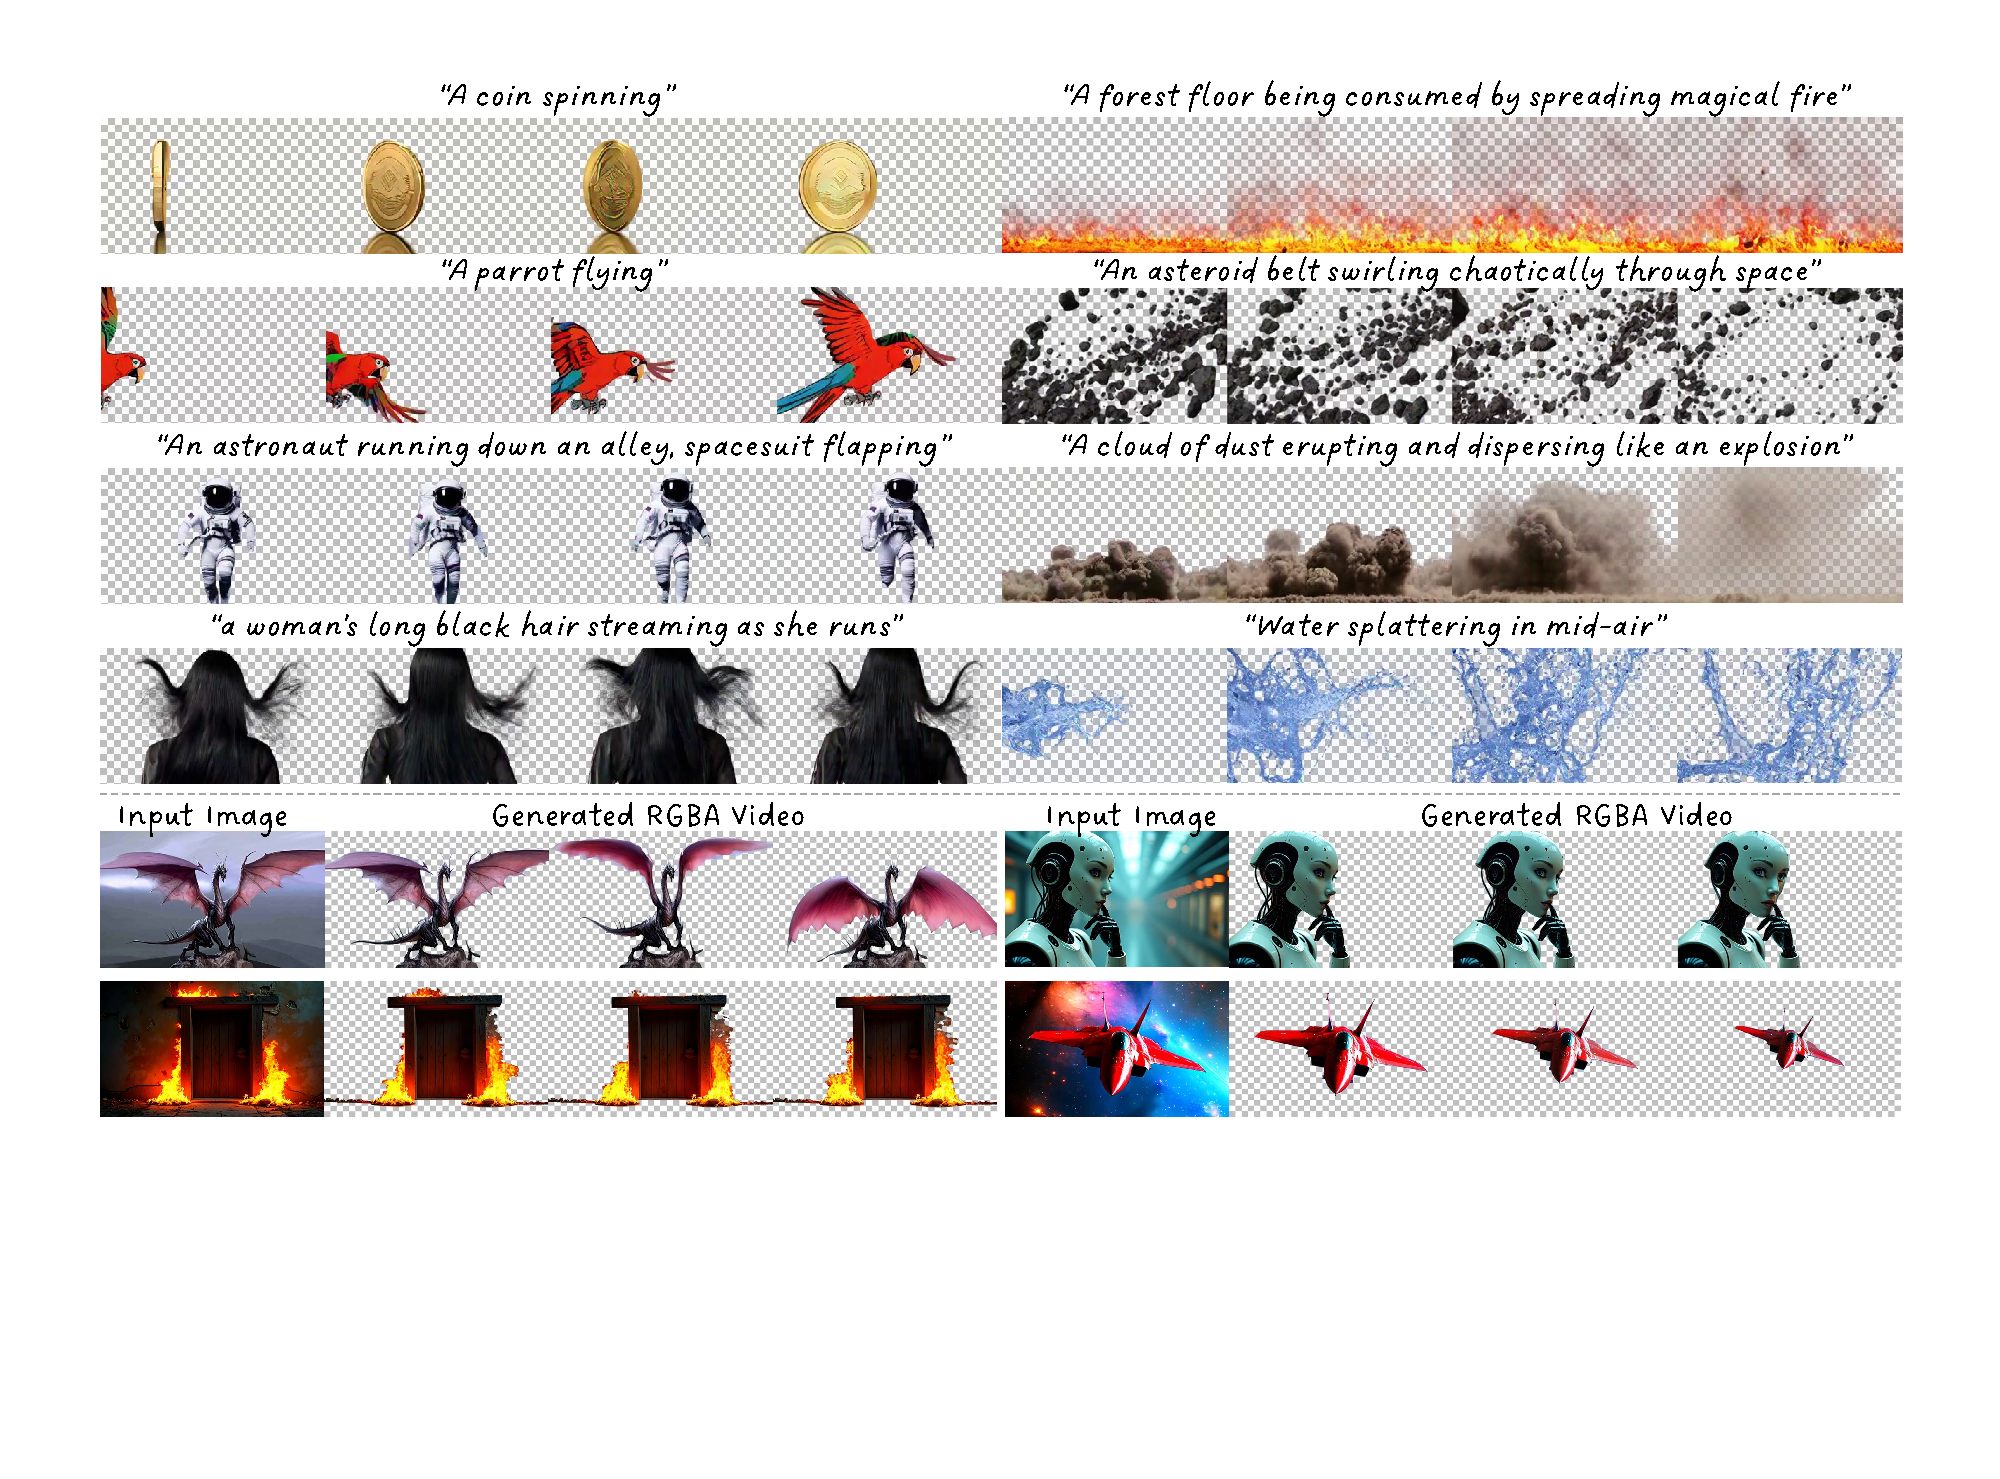
\includegraphics[width=1.0\linewidth]{figs/exp-applications.pdf}
    \vspace{-0.2in}
    \caption{\textbf{Applications.} \textbf{Top}: Text-to-Video with Transparency. \textbf{Bottom}: Image-to-Video generation with transparency.
.}
    \label{fig-applications}
    \vspace{-0.1in}
\end{figure*}


\section{Experiment}
\label{sec:exp}

%-------------------------------------------------------------------------
%\subsection{Implementation Details}

\noindent\textbf{Training Dataset.}~We utilize the public VideoMatte240K dataset~\cite{lin2021real}, a comprehensive collection of 484 high-resolution green screen videos consists of 240,709 unique frames of alpha mattes and foregrounds. These frames provide a diverse range of human subjects, clothing styles, and poses. We apply fundamental preprocessing steps for them, including color decontamination and background blurring. Prompts are extracted using ShareGPT4V~\cite{chen2023sharegpt4v}. 

\vspace{0.5em}
\noindent\textbf{Model.}~Our RGBA video diffusion models are developed by fine-tuning pre-trained diffusion models. Specifically, we employ two models based on the diffusion transformer architecture: the open-source model CogVideoX~\cite{yang2024cogvideox} and a modified variant of CogVideoX denoted as \(J\). 
CogVideoX generates RGB videos at a resolution of 480x720 with 49 frames at 8 FPS, using 50 sampling steps. In contrast, the modified version produces videos at a resolution of 176x320 with 64 frames at 24 FPS, while also using 50 sampling steps. Additionally, we integrate our method with CogVideoX-I2V (Image-to-Video) to support image-to-video generation with transparency.
We set the LoRA rank to 128. For domain embedding, we initialize it with an original shape of \(1\times D\) and zero values, then expand it to \(L\times D\) through repetition during training. 
We train these parameters over 5,000 iterations with a batch size of 8 in total, utilizing 8 NVIDIA A100 GPUs.



\begin{figure*}[htbp]
    \centering
    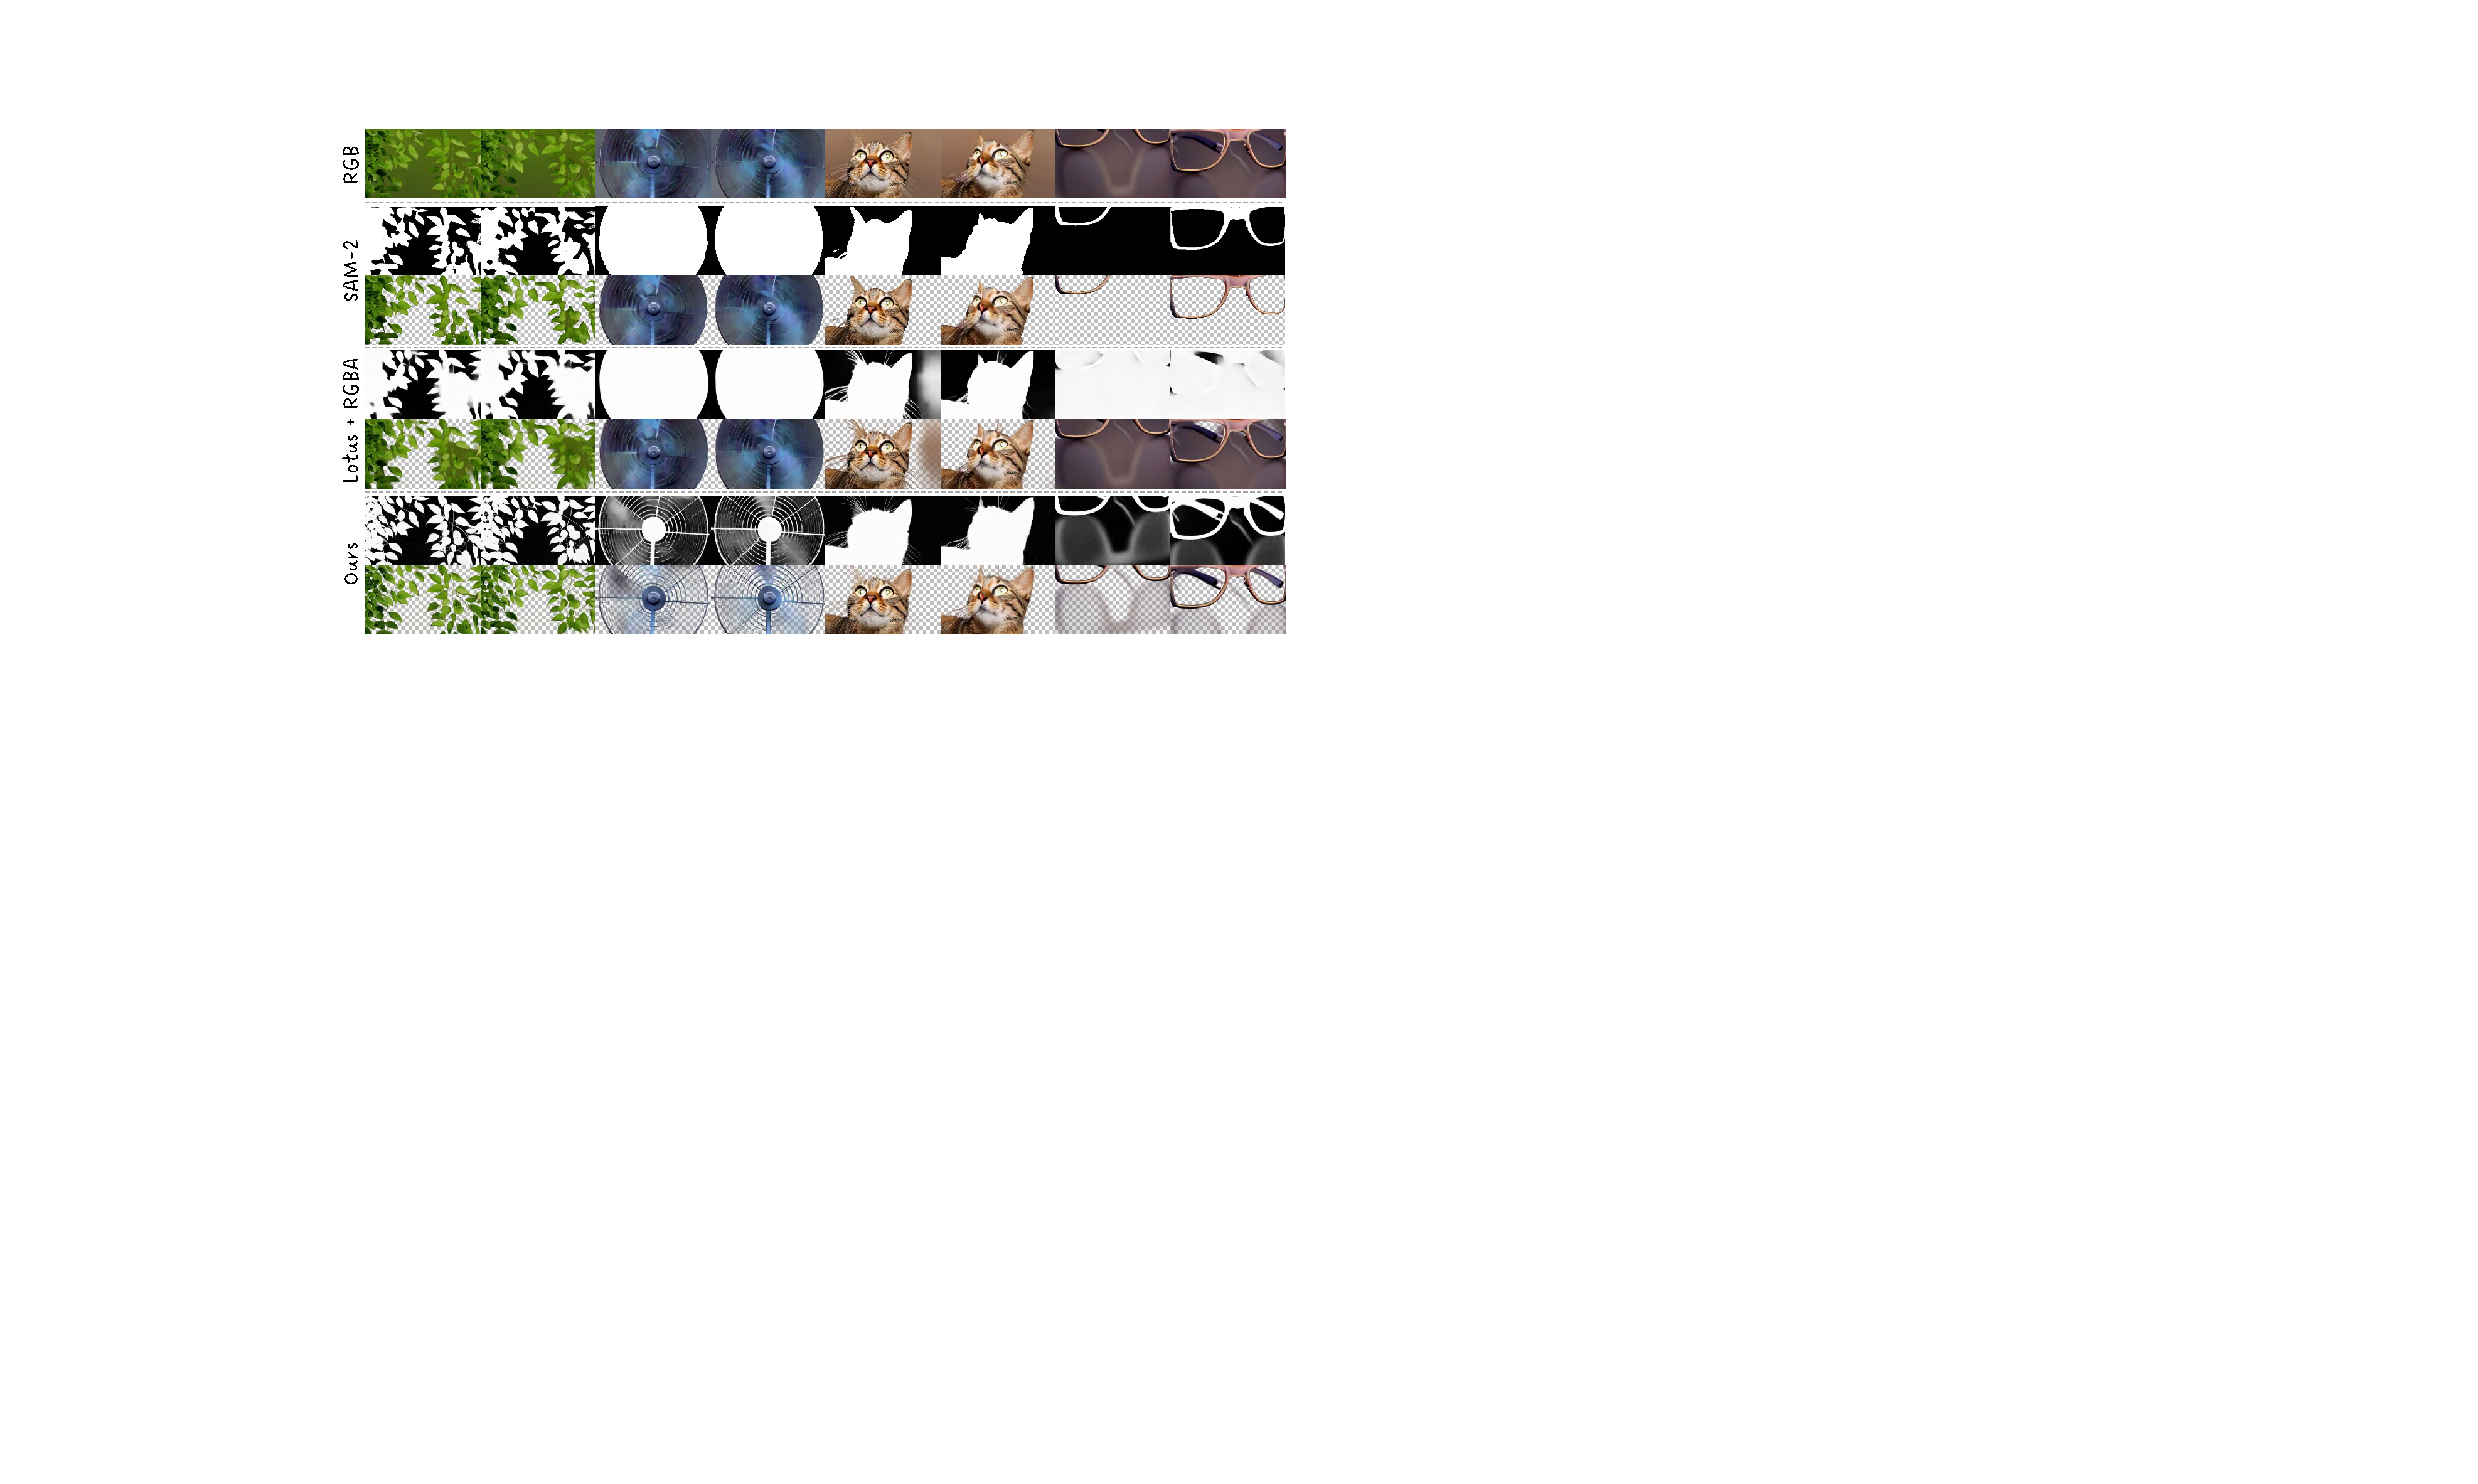
\includegraphics[width=1.0\linewidth]{figs/exp-comparison.pdf}
    \vspace{-0.2in}
    \caption{\textbf{Comparison with Generation-then-Prediction Pipelines.} Our method demonstrates superior alignment.
}
    \label{fig-comparison}
\end{figure*}

\begin{figure*}[htbp]
    \centering
    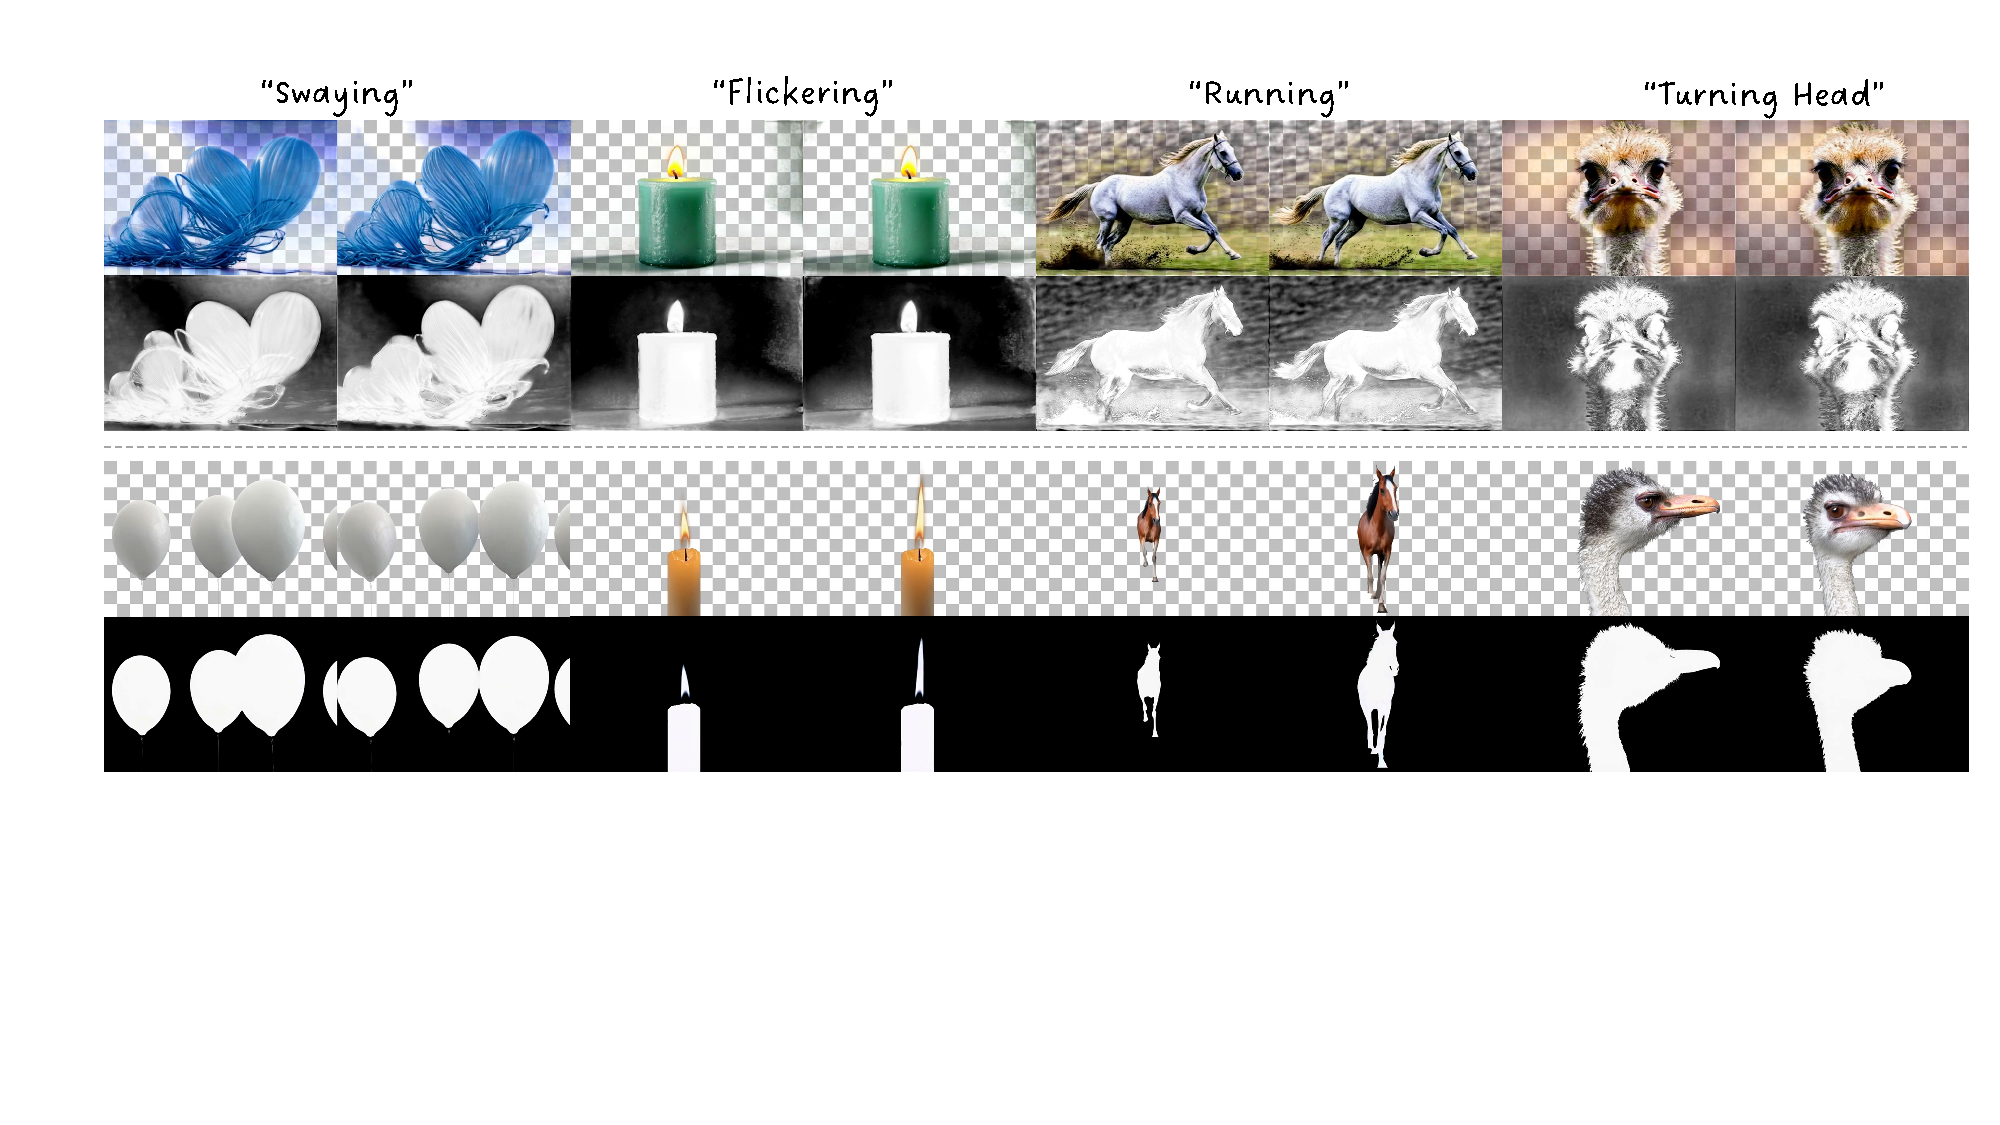
\includegraphics[width=1.0\linewidth]{figs/exp-comparison-generation.pdf}
    \caption{\textbf{Comparison with Joint Generation Pipelines.} \textbf{Top}: LayerDiffusion + AnimateDiff; \textbf{Bottom}: Ours. Our method achieves better alignment and generates corresponding motion described by prompts.}
    \label{fig-comparison-generation}
    \vspace{-0.1in}
\end{figure*}

% %-------------------------------------------------------------------------
\subsection{Applications}
We mainly demonstrate two applications shown in Fig.~\ref{fig-applications}: 

\vspace{0.5em}
\noindent\textbf{Text-to-Video with Transparency.}~Our method is capable of generating moving objects with various types of motion, such as spinning, running, and flying, while also handling transparent properties of bottles and glasses. Additionally, it can produce complex visual effects, including fire, explosions, cracking, and lightning, as well as creative examples.

\vspace{0.5em}
\noindent\textbf{Image-to-Video with Transparency.}~Our method can also be integrated with an I2V video generation model-CogVideoX-I2V. Users can provide a single image along with an alpha channel (optional), and then we generate subsequent frames with dynamic effects and automatically propagate or generate alpha channels for these frames.



% %-------------------------------------------------------------------------
\subsection{Comparisons}

% \noindent\textbf{Generation-then-Prediction Pipeline.}~We compare our method with a generation-then-prediction pipeline. We first run our approach, denoted as \( J \), to generate both RGB and alpha channels. Then, we apply various prediction models to infer the alpha channel based on the generated RGB frames. For our main baselines, we use Lotus~\cite{he2024lotus} and SAM-2~\cite{ravi2024sam2}, which either leverage pretrained RGB models or are trained on large datasets. Since Lotus was originally designed for single-image depth estimation, we adapt its framework for application within our video generation model (\( J \)). For comparisons with video matting methods~\cite{lin2021real,qin2023bimatting,yao2024matte}, which are trained exclusively on human portraits and lack generalizability to other objects, please refer to the supplementary materials.
\noindent\textbf{Generation-then-Prediction Pipeline.}~As shown in Fig.~\ref{fig-intro}, video matting methods~\cite{lin2021real,qin2023bimatting,yao2024matte} struggle with matting non-human objects (see supplementary materials for additional results). Therefore, we selected Lotus~\cite{he2024lotus} and SAM-2~\cite{ravi2024sam2} as baselines due to their stronger generalization: Lotus uses pretrained generative models, and SAM-2 is trained on large datasets. Since Lotus was originally designed for single-image depth estimation, we extended it for RGBA videos, denoted as Lotus + RGBA in our comparisons. Qualitative results are shown in Fig.~\ref{fig-comparison}. Since ground-truth alpha channels are not available for generated videos, we focus on qualitative comparison. 


\vspace{0.5em}
\noindent\textbf{Joint Generation Pipeline.}~Since there are currently no existing RGBA video generation models, we integrate AnimateDiff~\cite{guo2023animatediff} with LayerDiffusion~\cite{zhang2024transparent} to generate RGBA videos. We use the open-source video generation model CogVideoX~\cite{yang2024cogvideox} as the base model for fair comparison. 
The qualitative results are illustrated in Fig.~\ref{fig-comparison-generation}.


\vspace{0.5em}
\noindent\textbf{User Study.}~
We also conduct a user study with Amazon Mechanical Turk to compare two joint generation methods, as shown in Table.~\ref{tab:user_study}. Participants are asked to evaluate two key aspects: 1) whether the RGB and alpha align correctly; and 2) whether the motion in the generated video matches the corresponding text description. A total of 30 videos are generated from distinct text prompts, and 87 users participated in the evaluation. The study shows that our method is obviously favored more by users with higher votes.

\begin{table}
    \centering
    \caption{\textbf{User Study.}}
    \vspace{-0.1in}
    \resizebox{1.0 \columnwidth}{!}{%
    \begin{tabular}{ccc} \toprule
         &RGBA Alignment  &Motion Quality \\ \toprule AnimateDiff~\cite{guo2023animatediff}+LayerDiff~\cite{zhang2024transparent}& 6.7\% &21.7\% \\ 
         Ours + CogVideoX~\cite{yang2024cogvideox}& \textbf{93.3\%} &\textbf{78.3\%} \\ \bottomrule
    \end{tabular}
    }
    \vspace{-0.1in}
    \label{tab:user_study}
\end{table}



% %-------------------------------------------------------------------------
\subsection{Ablation Study}
\begin{figure}[htbp]
    \centering
    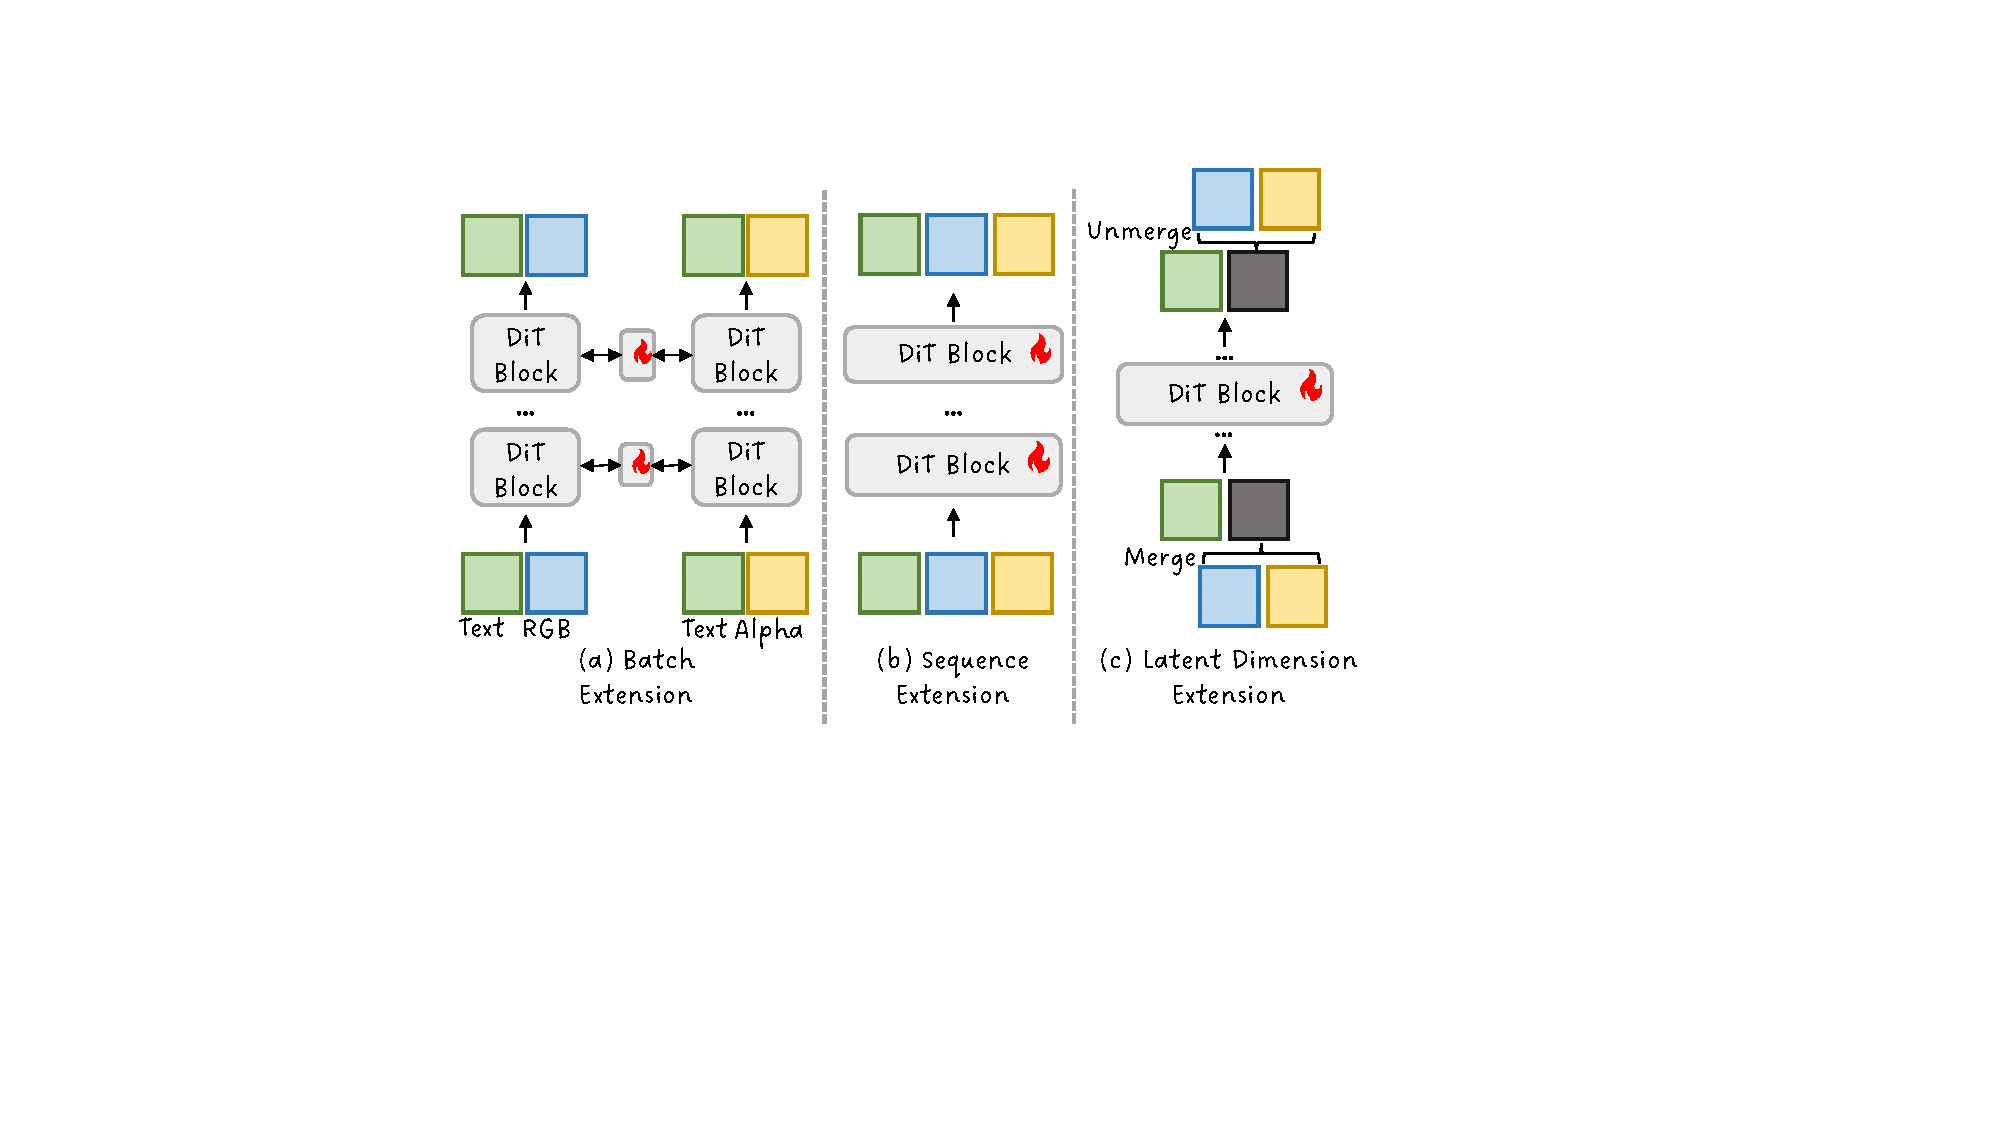
\includegraphics[width=1.0\linewidth]{figs/discussions.pdf}
    \caption{\textbf{Alternative Designs for Joint Generation with DiT}. Sequence extension (b) represents our method.}
    \label{fig-arch}
\end{figure}
As shown in Fig.~\ref{fig-ablation}, we conduct the ablation study across two dimensions: attention rectification and network design.
\begin{figure}[h]
    \centering
    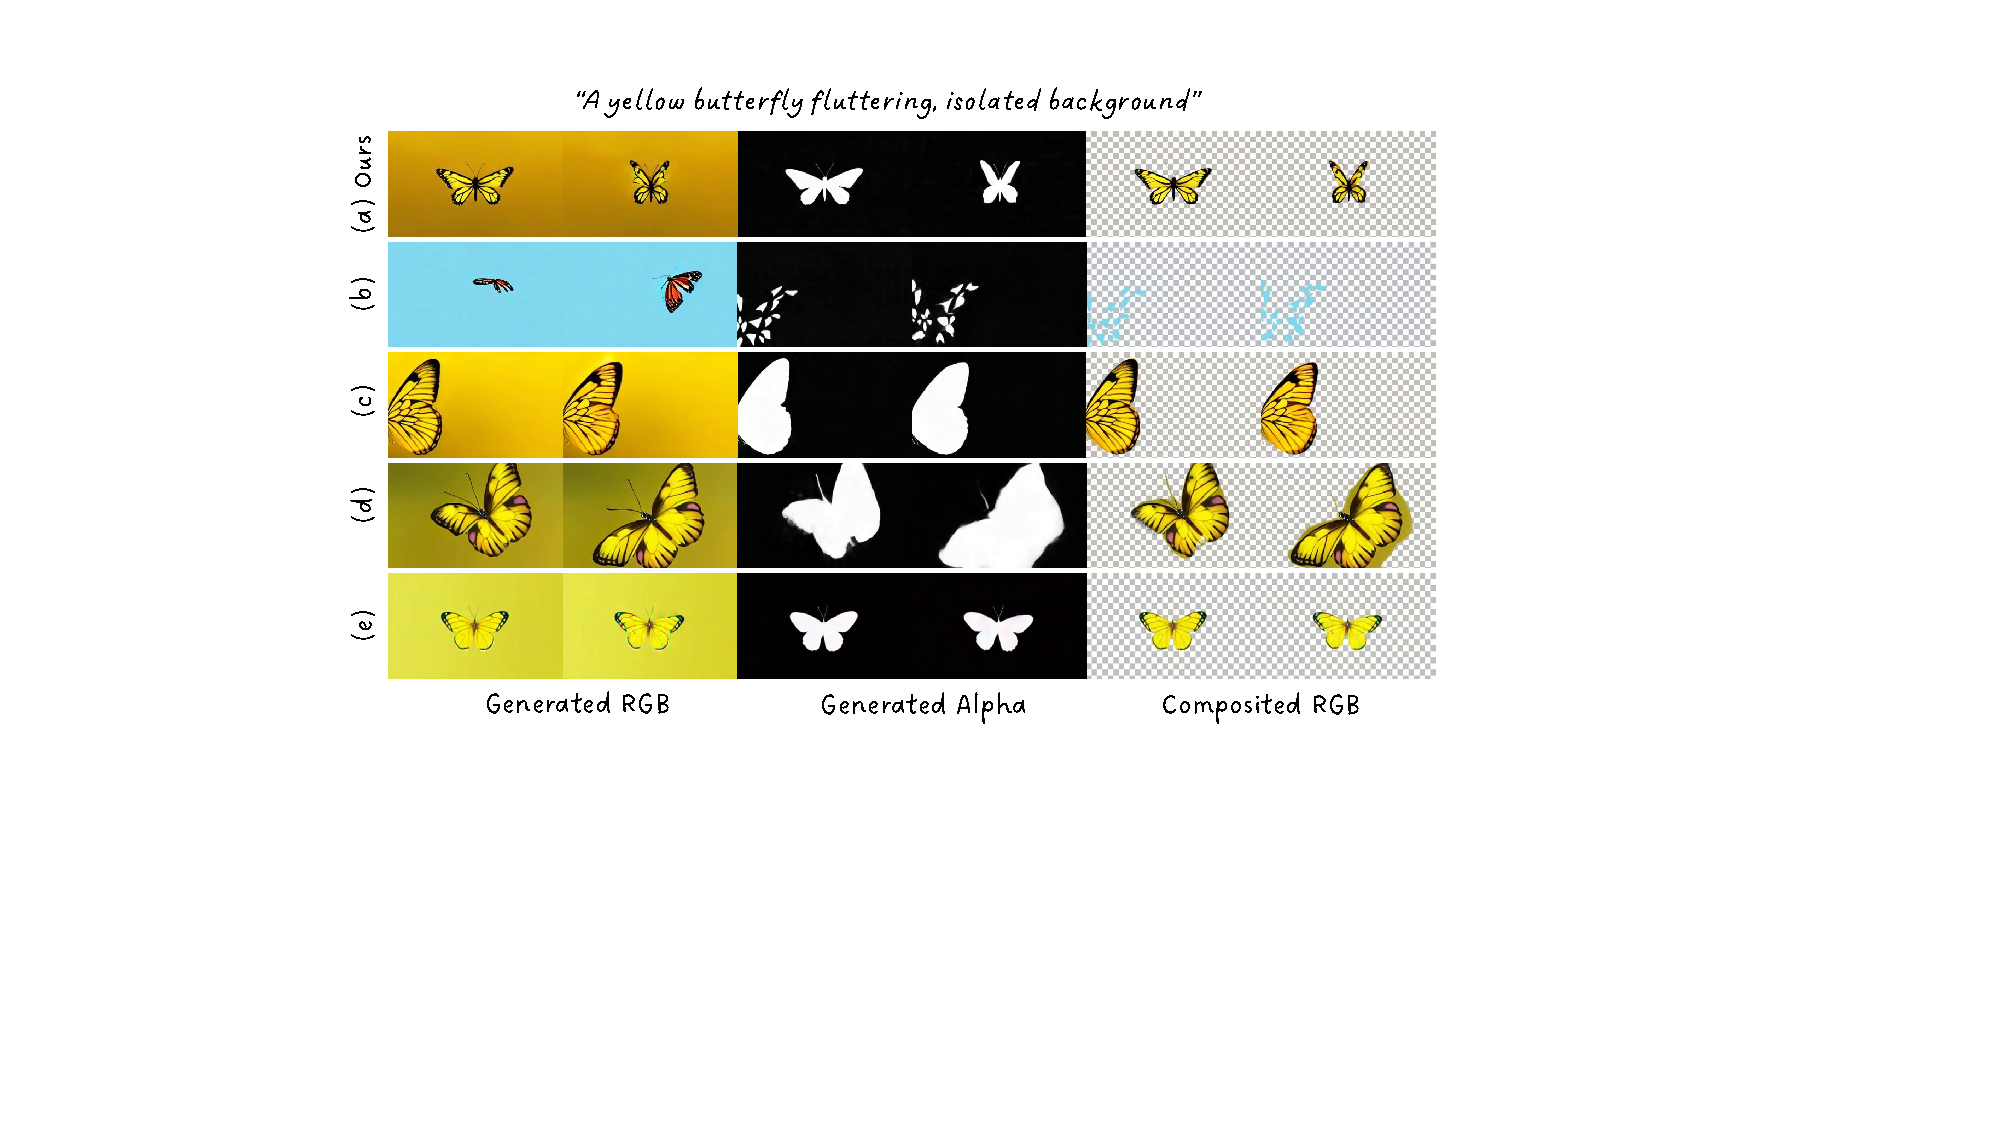
\includegraphics[width=1.0\linewidth]{figs/exp-ablation.pdf}
    \caption{\textbf{Ablation Study.} (a) Ours; (b) Ours without RGB-attend-to-Alpha; (c) Ours with Text-attend-to-alpha; (d) Batch Extension Strategy; (e) Latent Dimension Extension Strategy. Our method maintains high-quality motion generation (e.g., butterflies waving their wings) while achieving good alignment.}
    \label{fig-ablation}
\end{figure}


\vspace{0.5em}
\noindent\textbf{Attention Rectification.}~
By blocking RGB-to-Alpha attention, we first validate the importance of RGB-to-Alpha attention for aligning RGB and alpha channels, a feature lacking in most prediction-based methods. We also examine the effect of removing unnecessary attention to preserve the model's generative capacity, by learning Text-to-Alpha attention only.
Without RGB-to-Alpha attention, the alpha channel misaligns with RGB content %causing background artifacts. %When only Text-to-Alpha attention is used, 
and the RGB output loses motion quality (e.g., reverse rocket).

\vspace{0.5em}
\noindent\textbf{Alternative Designs For Joint Generation.}~
Given the transformer’s input dimensions \( B \times L \times D \), we extend the sequence dimension \( L \) to produce RGB and alpha channels, but alternative extensions are possible at the Batch \( B \) or Latent Dimension \( D \) levels (see Fig.~\ref{fig-arch}). In the \textbf{Batch Extension} approach, a new module enables inter-batch communication, similar to the technique in~\cite{vainer2024collaborative}. For \textbf{Latent Dimension Extension}, we merge video and alpha tokens, project them into the DiT model’s latent space, and unmerge post-generation, using learnable linear layers with fine-tuning. Batch Extension shows weaker RGB-alpha alignment, while Latent Dimension Extension, though akin to training from scratch, significantly reduces diversity.

\vspace{0.5em}
\noindent\textbf{Evaluation.}~
In addition to the qualitative comparisons shown in Fig.~\ref{fig-ablation}, we also generated a total of 80 videos, each consisting of 64 frames, and evaluated them using two primary metrics:
\textbf{Flow Difference.} To measure alignment between the generated RGB and Alpha videos, we use optical flow~\cite{horn1981determining} to focus on motion consistency while ignoring appearance. Specifically, we calculate optical flow with Farneback method~\cite{farneback2003two} and compute the flow difference as the average Euclidean distance between RGB and Alpha flow fields.
\textbf{Frechét Video Distance (FVD).} We use FVD~\cite{unterthiner2019fvd} to compare the RGB videos generated by each RGBA method against those from the original RGB model, evaluating how well each method preserves the model's original generative quality. A lower FVD indicates that the generated results are closer to the original RGB model in terms of motion coherence and diversity, thus demonstrating a high fidelity to the model's intended generative quality.
Results are shown in Fig.~\ref{fig-abaltion-metrics}.

\begin{figure}[t]
    \centering
    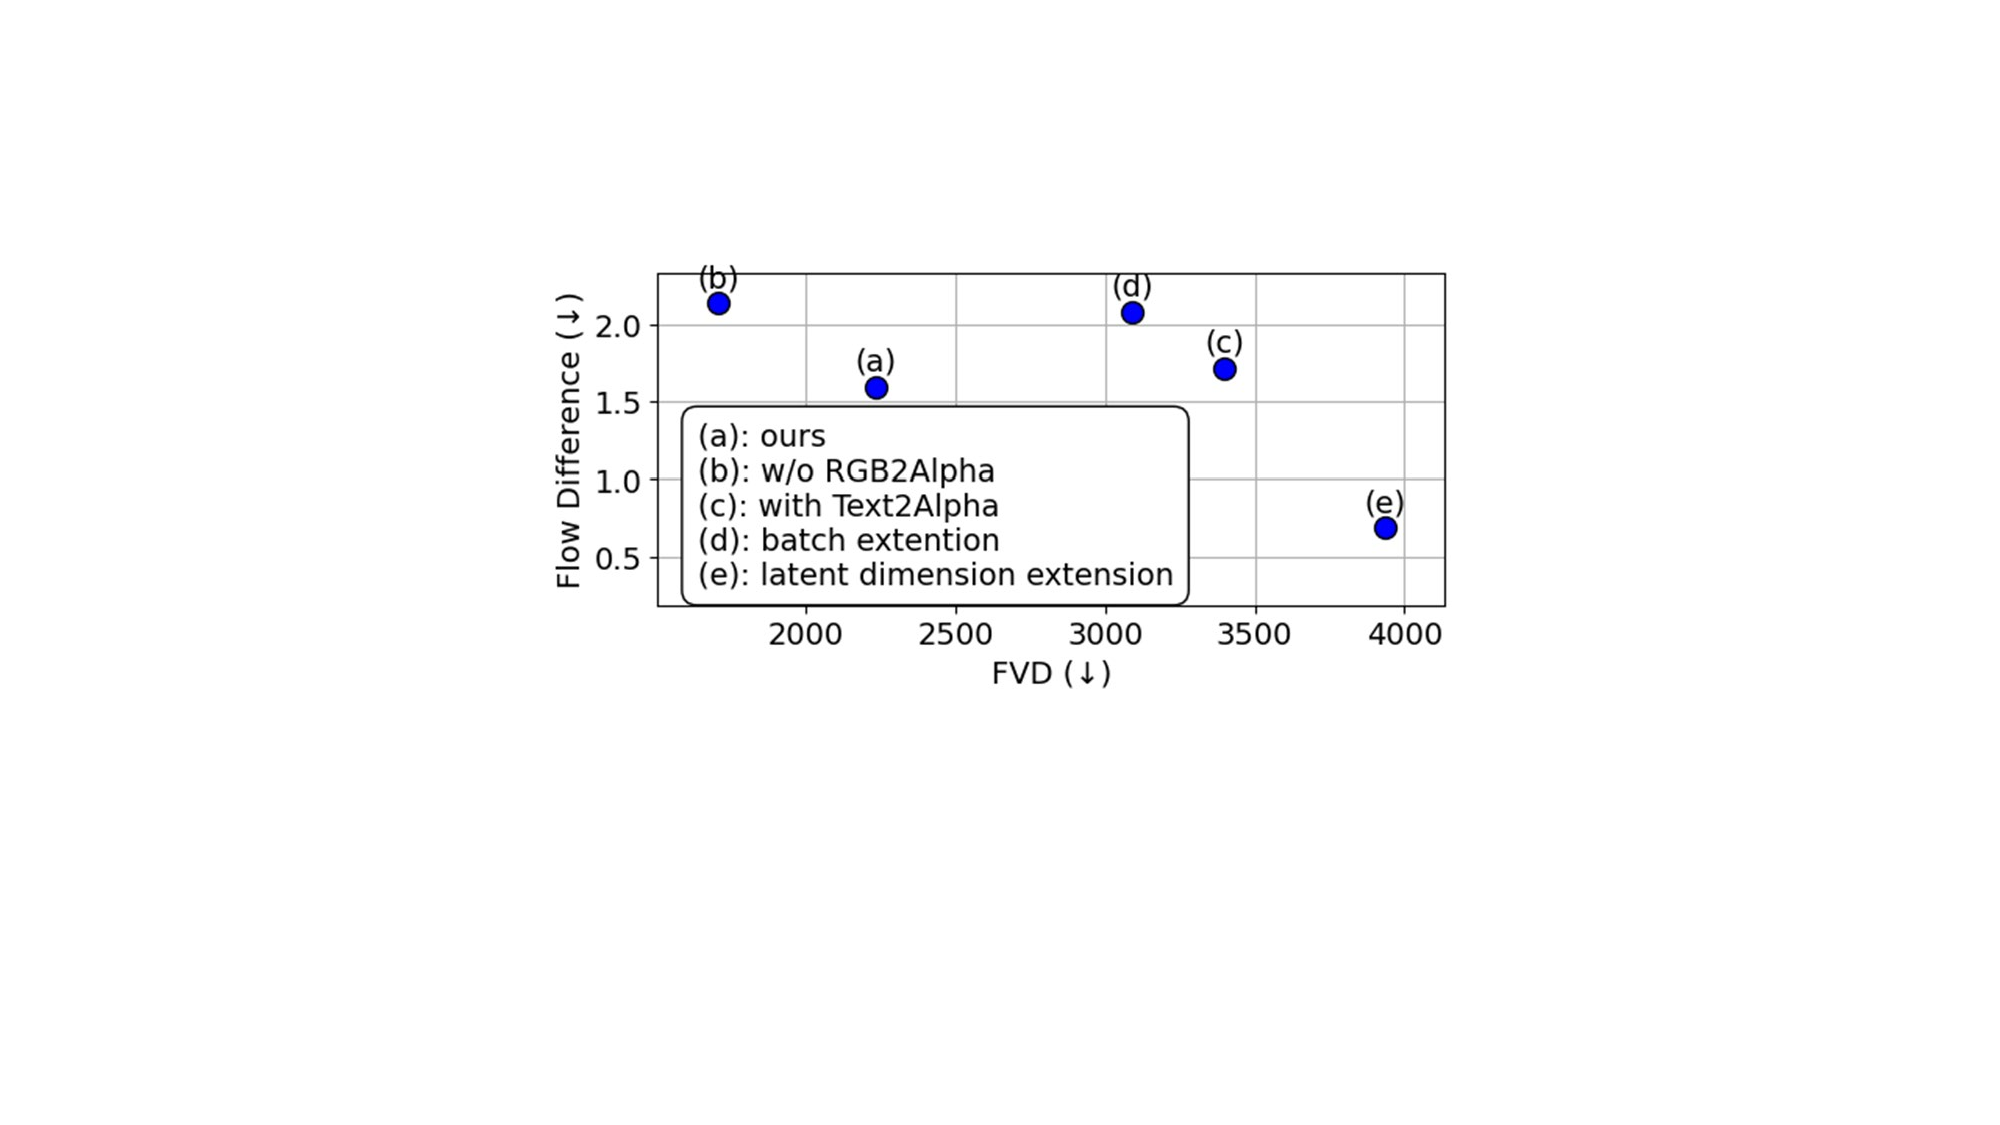
\includegraphics[width=0.9\linewidth]{figs/exp-ablation-metrics}
    \vspace{-0.1in}
    \caption{\textbf{Quantitative Evaluation}. Our approach achieves a good balance between alignment (low flow difference) and preserving generative quality (low FVD).}
    \label{fig-abaltion-metrics}
    \vspace{-0.1in}
\end{figure}
% %-------------------------------------------------------------------------
%\subsection{Limitations}
% \vspace{0.5em}
% \noindent\textbf{Limitation.} Our transformer-based method for RGBA generation incurs quadratic computational costs due to sequence expansion. However, it achieves strong results on a limited dataset. Also, numerous studies have addressed the computational overhead of long sequences, with many optimizations reducing complexity to a linear scale. To enhance the efficiency of our method, we plan to incorporate these optimizations in future work. %Additionally, our performance is shaped by the generative priors provided by the T2V model, which influence the quality and consistency of our outputs.











\section{Conclusion}
\label{sec:conclusion}
In this paper, we have investigated the common and unresolved issue that many established neural networks suffer from low floating-point operations per second (FLOPS). We have revisited a bottleneck operator, DWConv, and analyzed its main cause for a slowdown -- frequent memory access. To overcome the issue and achieve faster neural networks, we have proposed a simple yet fast and effective operator, PConv, that can be readily plugged into many existing networks. We have further introduced our general-purpose FasterNet, built upon our PConv, that achieves state-of-the-art speed and accuracy trade-off on various devices and vision tasks. We hope that our PConv and FasterNet would inspire more research on simple yet effective neural networks, going beyond academia to impact the industry and community directly.


% WARNING: do not forget to delete the supplementary pages from your submission 
\clearpage

\setcounter{page}{1}
\maketitlesupplementary

% \section{Supplementary video}
% Please see the supplementary video for an overview of our paper and for additional visualizations.

\section{\dataset Statistics}
We collected around 110k clips from 6,493 Internet VR180 videos.
\Fig{supp:camera_stats} shows the camera translation distribution between the first and last frame of each clip. 
In \Fig{supp:motion_stats}, we measure the motion in terms of pixel displacement projected onto the image frame. Measuring motion in pixel-space emphasizes motion that occurs closer to the camera, since such motion yields larger pixel displacements, while naturally de-emphasizing motion further from the camera. 

\section{More qualitative comparisons}
% Please see the supplementary video for additional visual examples of data in \dataset.


\subsection{More results on held-out  \dataset examples}
\Fig{supp:qualitative-stereo4d} shows additional \method predictions on the \dataset held-out test set, extending \Fig{result-wall-stereo4dtest} from the main paper. \Fig{supp:compare-stereo4d} shows additional qualitative examples of motion comparisons on \dataset test set, extending~\Fig{compare-stereo4d} from the main paper. \Fig{supp:compare-stereo4d} compares variants of DynaDUSt3R trained on different data sources. The model trained on PointOdyssey incorrectly predicts large 3D motions, while the model trained on Stereo4D makes more accurate motion predictions, closer to ground truth.

\begin{figure}[t]
    \centering
    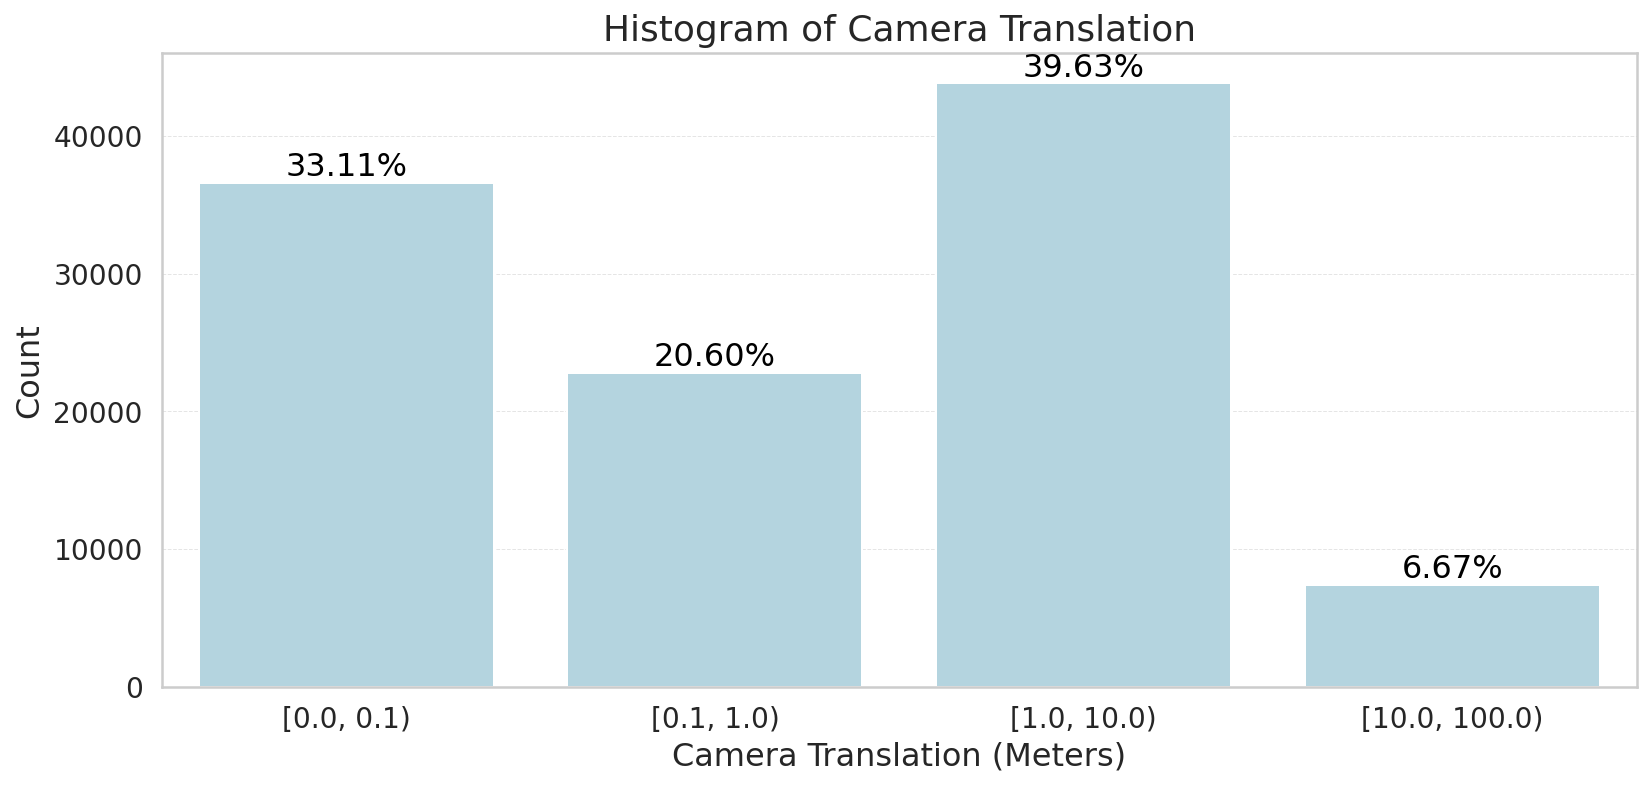
\includegraphics[width=\linewidth]{fig/supp/camera_stats.png}
    \caption{Camera statistics from \dataset. We measure the difference (in meters) of camera poses between the start and end frame of each video clip as calculated by SfM.}
    \label{fig:supp:camera_stats}

    \centering
    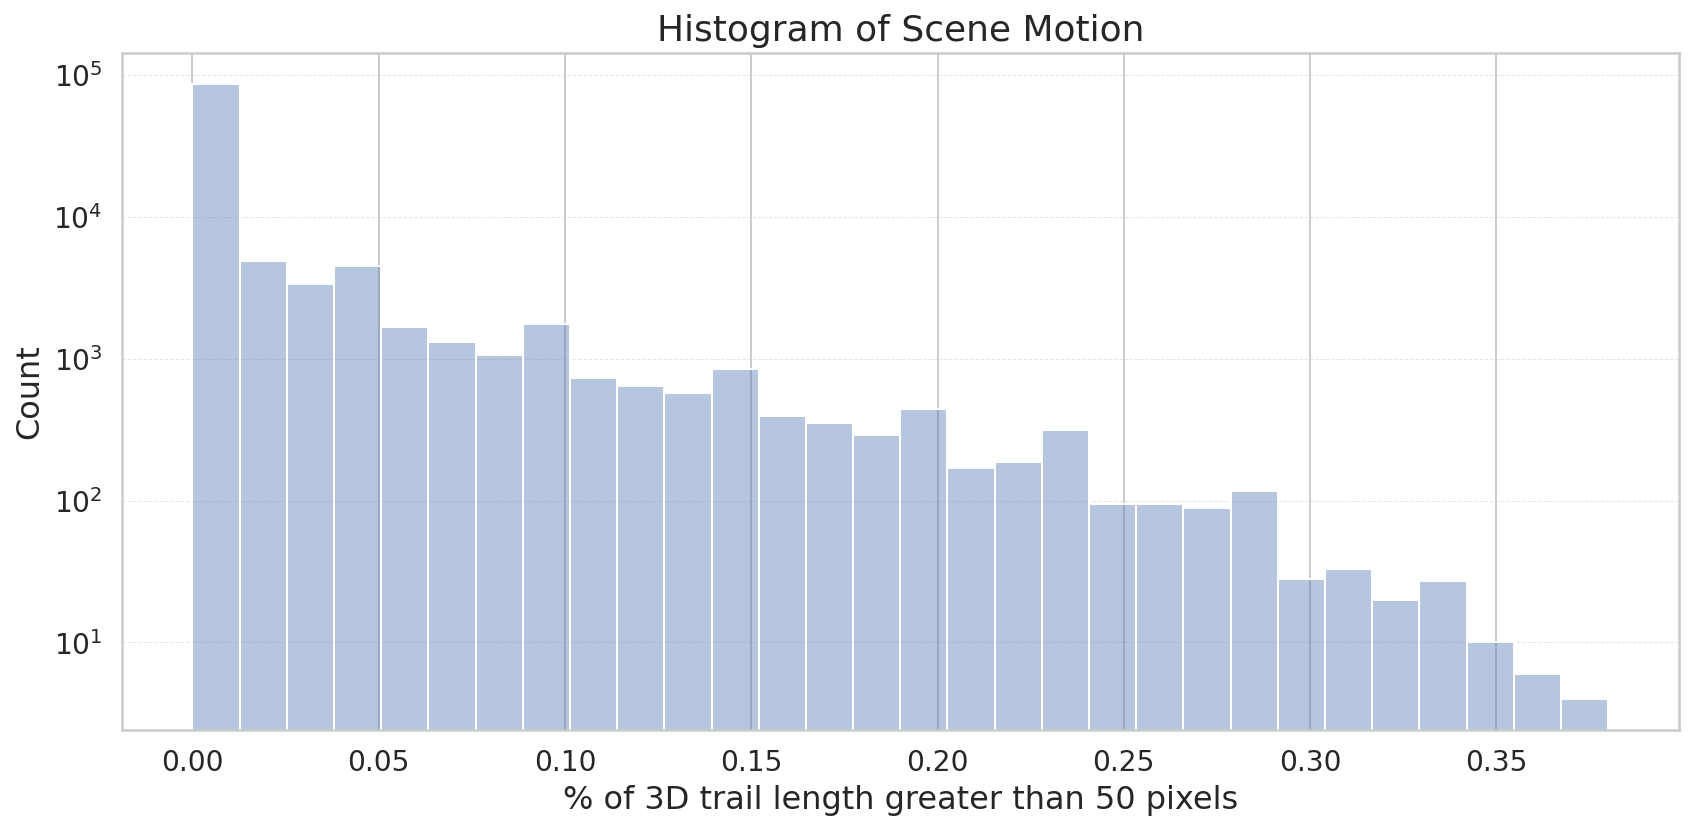
\includegraphics[width=\linewidth]{fig/supp/track_stats.png}
    \caption{Scene motion statistics from \dataset. We measure the motion in terms of pixel displacement projected onto the image frame. For each video, we measure the percentage of tracks that have 3D trail length greater than 50 pixels. The 3D trail length is measured by Eqn.~\ref{eqn:trail_length_def}. }
    \label{fig:supp:motion_stats}
\end{figure}

\begin{figure*}[ht]
    \centering
    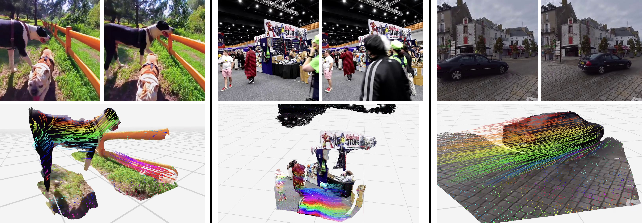
\includegraphics[width=\textwidth]{fig/supp/qualitative-stereo4d.pdf}
    \caption{\textbf{More qualitative results on \dataset test set.} Extending~\Fig{result-wall-stereo4dtest}, we visualize image pairs and corresponding dynamic 3D point clouds predicted by DynaDUSt3R trained on \dataset. Our method recovers accurate 3D shape and complex scene motion.}
\label{fig:supp:qualitative-stereo4d}
\end{figure*}

\begin{figure*}[ht]
    \centering
    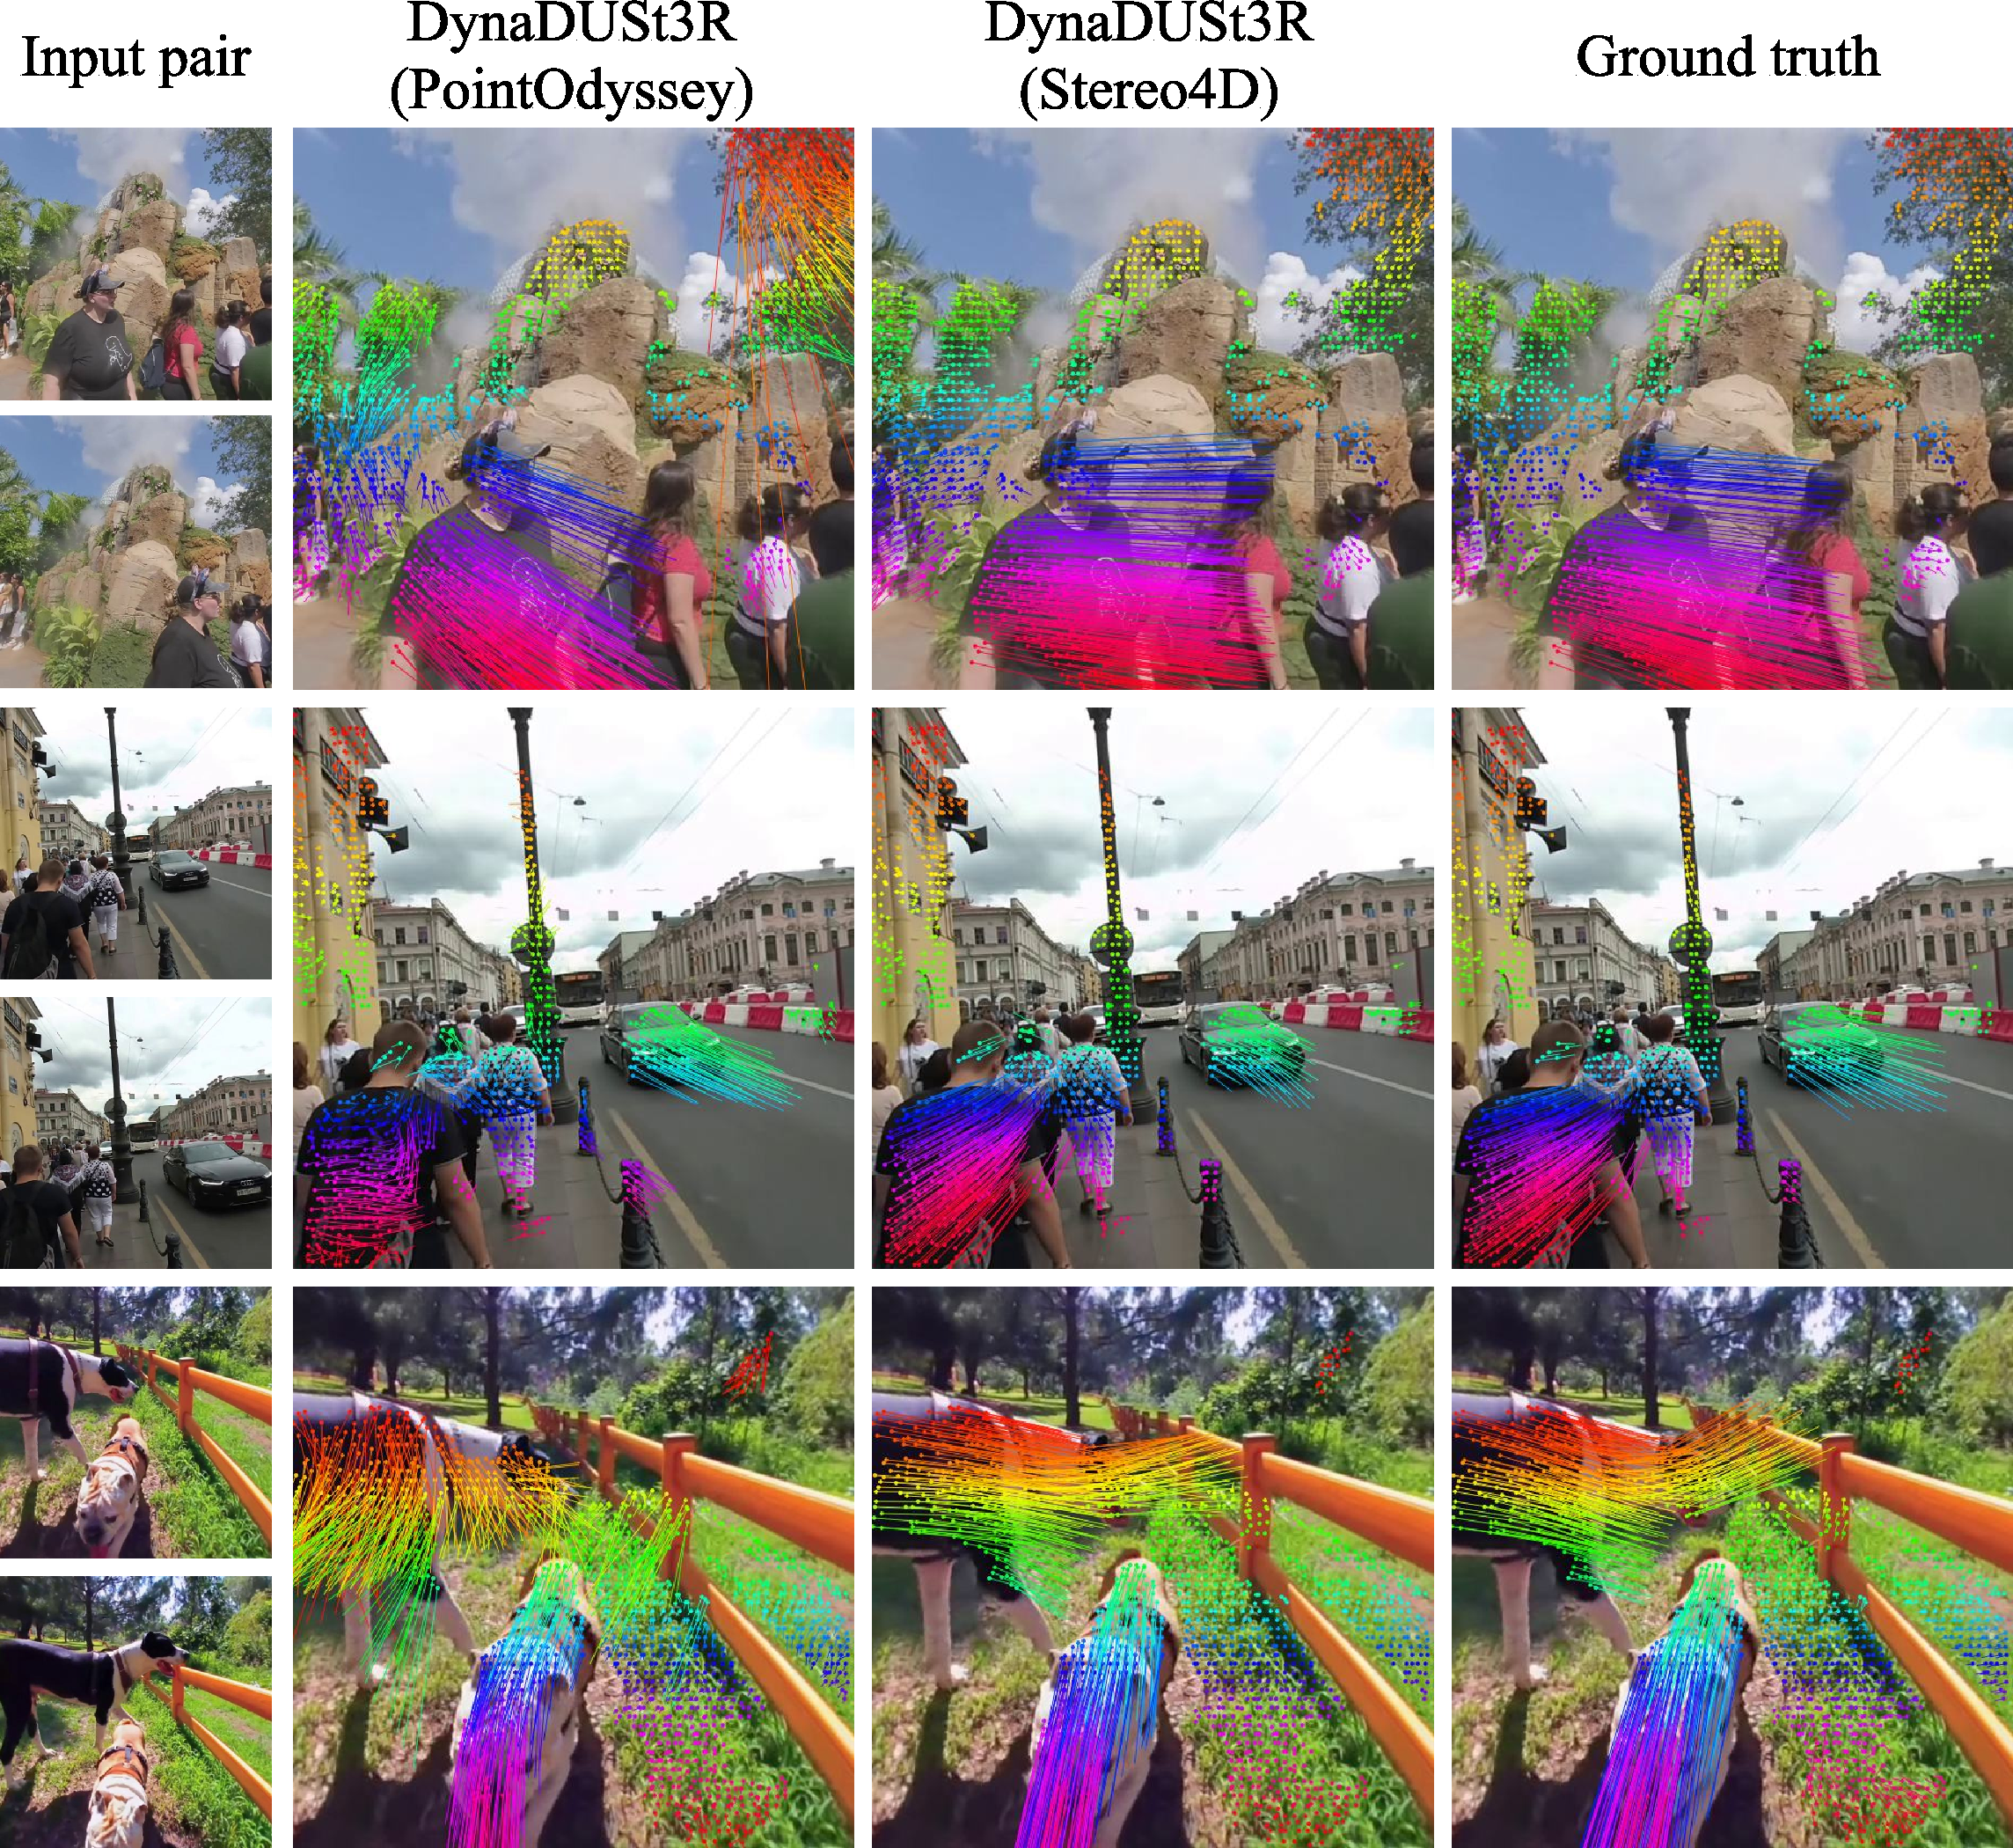
\includegraphics[width=\textwidth]{fig/supp/qualitative_comparison_on_motion_stereo4d.pdf}
    \caption{\textbf{More qualitative comparisons of 3D motion in the \dataset test set.} Extending~\Fig{compare-stereo4d}, we compare variants of DynaDUSt3R trained on different data sources. The Stereo4D-trained model also makes more precise motion predictions than the PointOdyssey-trained model.}
\label{fig:supp:compare-stereo4d}
\end{figure*}



\subsection{More qualitative examples on track optimization}
In \Fig{supp:track_comparison}, we illustrate estimated tracks for a video sequence featuring a forward-moving camera and vehicles driving towards the camera. Our initial 3D tracks derived directly from RAFT depth, BootsTAP 2D tracks, and SfM camera pose, show significant jitter for both dynamic (vehicle) and static (ground) points. 
However, after applying our track optimization, the ground points produce stable, static tracks, and vehicle tracks become smooth and coherent. 

\begin{figure*}[ht]
    \centering
    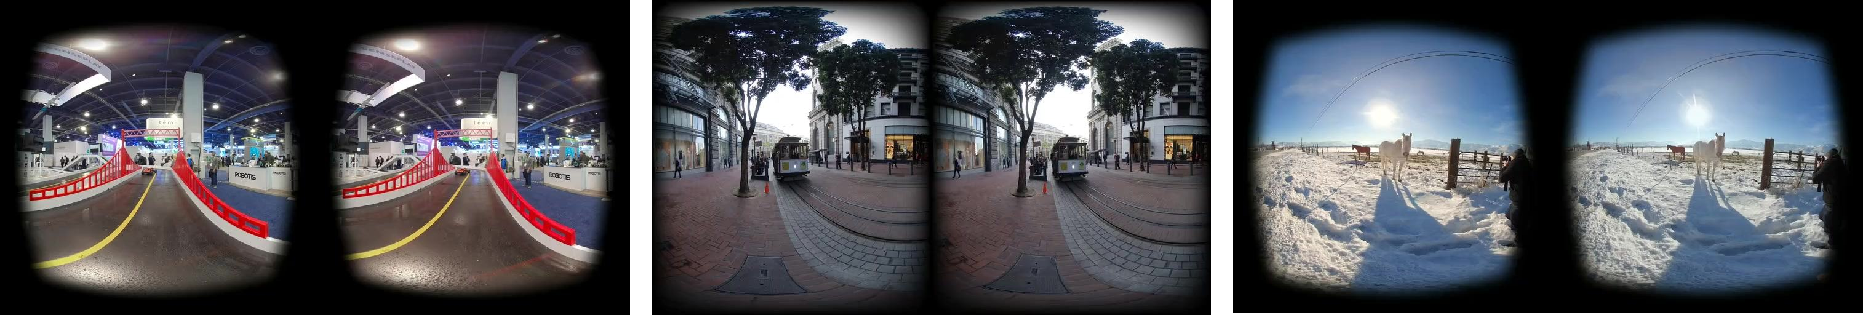
\includegraphics[width=\textwidth]{fig/supp/equirect-sample.pdf}
    \caption{Example equirectangular stereo videos collected from the internet.}
    \label{fig:supp:equirect}
\end{figure*}


\begin{figure*}[ht]
    \centering
    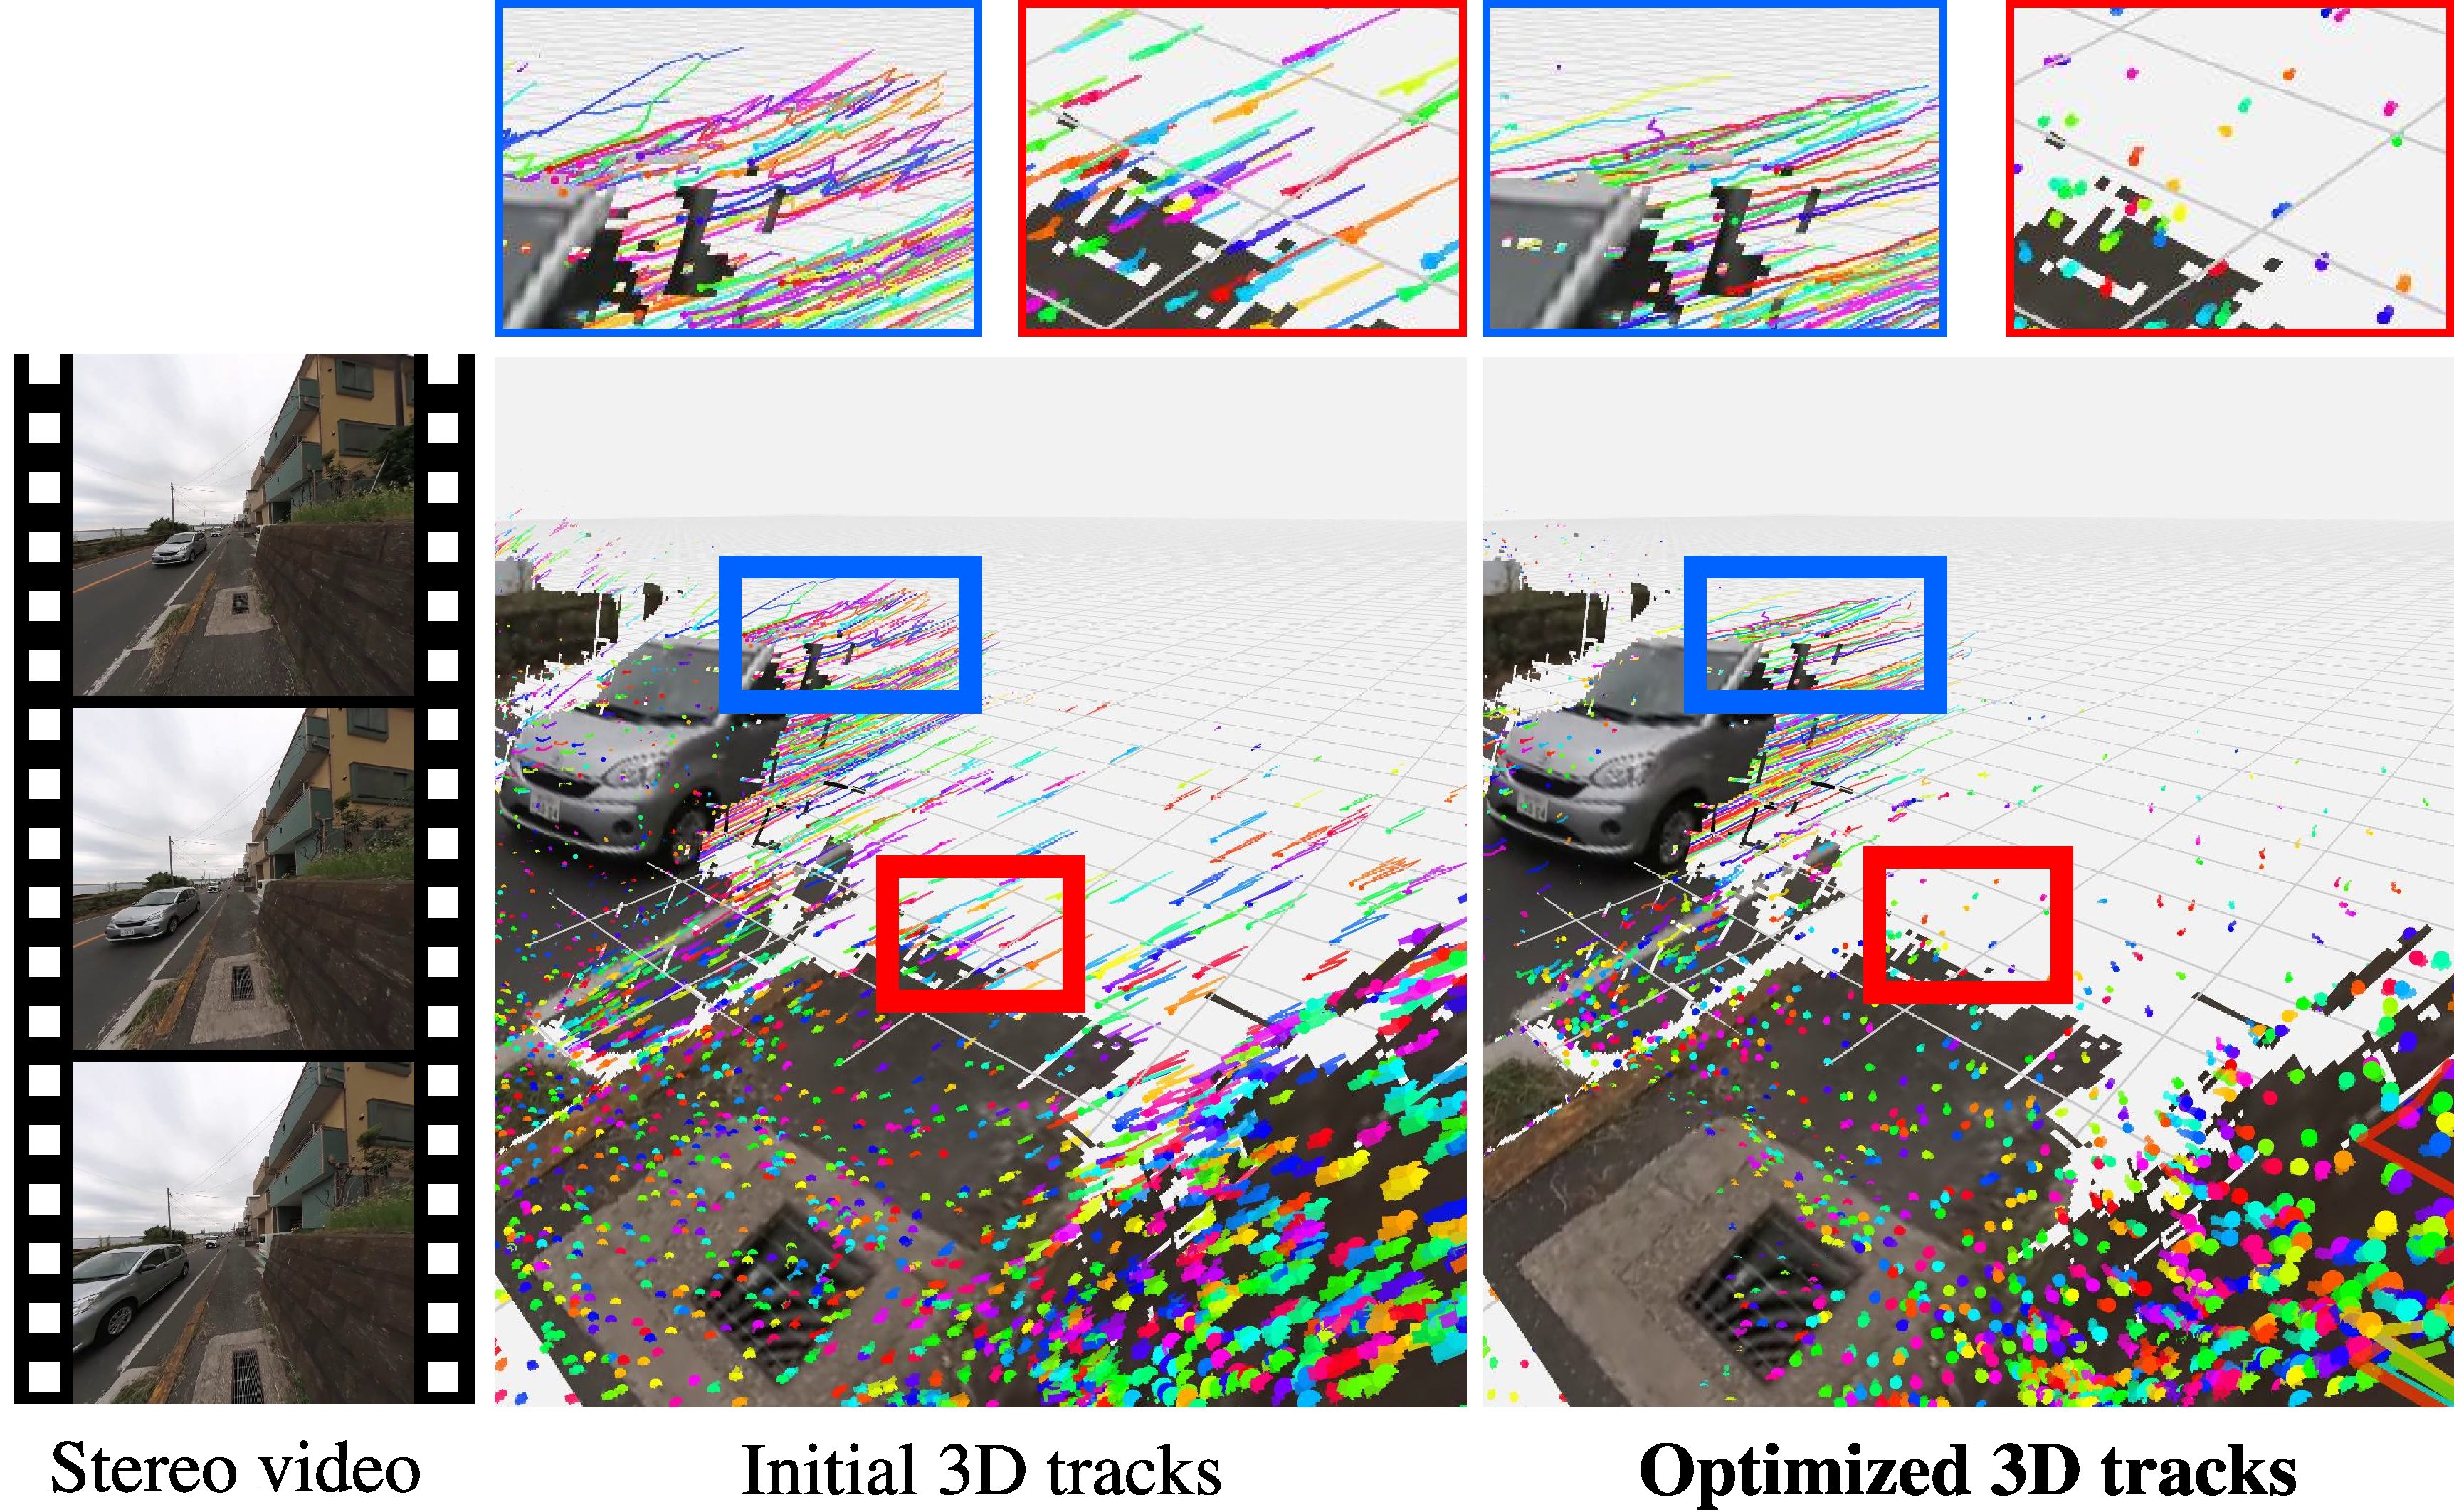
\includegraphics[width=0.8\textwidth]{fig/supp/track_optimization_car_comparison-2.pdf}
    \caption{\textbf{Effect of Track Optimization.} We compare 3D tracks on a challenging walking tour video sequence. In this clip (left), the camera moves forward while vehicles drive toward the camera. We visualize the results across 16 frames, showing 3D trails left by both dynamic and static points.  \textbf{Middle}: Our initial 3D tracks, created directly from RAFT, BootsTAP and SfM camera pose, also exhibit significant jitter for both dynamic (vehicle) and static (ground) points.  \textbf{Right}: After applying our track optimization, the ground points yield stable, static tracks, and vehicle tracks become smooth and coherent.}
\label{fig:supp:track_comparison}
\end{figure*}

\section{Dataset curation details}
\subsection{Equirectangular videos}
The raw videos that we collect (see examples in \Fig{supp:equirect}) are natively stored in a cropped equirectangular format, which differs from a full 360$^\circ$ equirectangular projection as the horizontal field of view of the cropped format typically spans 180$^\circ$---half of a full sphere. These videos often contain metadata specifying the horizontal and vertical field of view. 
For instance, metadata for a typical video might specify 
$\mathsf{start_{yaw}}=-90.0^\circ$, $\mathsf{end_{yaw}}=90.0^\circ$,  $\mathsf{start_{tilt}}=-90.0^\circ$, $\mathsf{end_{tilt}}=90.0^\circ$; 
Since many VR180 videos are designed for an immersive VR experience, they are typically viewed with headsets. Hence, the baseline between the left and right cameras typically closely matches the average human eye distance of 6.3 cm.


\subsection{SfM}
For ease of processing with standard 3D computer vision pipelines, and to benefit from the wide FoV of the input videos, we convert the videos from their native format (equirectangular projections) to a fisheye format for camera pose estimation. 
We use a 140$^\circ$ field of view for these fisheye-projected videos, because many equirectangular videos have a black fade-out/feathering/vignetting effect applied at the boundary, as shown in~\Fig{supp:equirect}.
We found that using wider FoV frames significantly improves camera pose estimation in dynamic scenes. 
When using narrow FoV projections, dynamic objects are more likely to occupy a large fraction of the frame; when these dynamic foreground objects are rich in features, they can confuse camera tracking algorithms, leading to inaccurate camera poses that track the dynamic object rather than producing true camera motion with respect to the environment. 
In contrast, wide-angle fisheye videos capture more background regions, which tend to have stable features for tracking, yielding more reliable camera poses.

We first use ORB-SLAM2's stereo estimation mode~\cite{murartal2015orbslam}
to identify trackable sequences within the videos, utilizing the method devised by Zhou \etal to divide videos into discrete, trackable shots~\cite{zhou2018stereo}. 
For each given shot, consisting of frames $(I_i, \ldots, I_n)$, we estimate camera poses and rig calibration via an incremental global bundle adjustment algorithm similar to COLMAP~\cite{schonberger2016structure}. 
We initialize the stereo rig calibration to be that of a rectified stereo pair with baseline 6.3 cm, but optimize for the calibration as part of the bundle adjustment process, as in practice the stereo rig can vary significantly from its nominal configuration.
This process yields a camera position $\mathbf{c}_i$ and orientation $\mathbf{R}_i$ for each frame $i$ (defined as the pose of the left camera), and a position $\mathbf{c}_r$ and orientation $\mathbf{R}_r$ for the right camera relative to the left (assumed to be constant throughout the shot).


\subsection{Depth estimation}
Depth estimation is first performed on a per-frame basis, with disparity maps computed independently for each frame.  

We use the estimated camera rig calibration $\cB_r, \RB_r$ to rectify the original  high resolution equirectangular video frames, ensuring that (1) the left and right views have centered principal points, (2) are oriented perpendicular to the baseline, and (3) pointing in a parallel direction.  We then convert the equirectangular videos to  perspective projections for downstream predictions.

Disparity is estimated from optical flow~\cite{teed2020raft, sun2022disentangling} between the rectified left and right frames. 
The $x$-component of the optical flow is used as disparity, which is converted to metric depth using:
\begin{equation}
    \mathsf{Depth} = \frac{\mathsf{baseline}  \times f}{\mathsf{disparity}}.
\end{equation}
Here $\mathsf{baseline}=0.063$m, and $f$ is the frame's focal length.

\medskip
\noindent \textbf{Outlier Rejection.} Several criteria are applied to filter out unreliable pixels: \emph{Inconsistency between left and right eyes:} Disparity is rejected if the optical flow fails a cycle-consistency check with an error exceeding one pixel. \emph{Depth values exceeding 20 meters} are considered invalid. Estimating accurate depth beyond a certain range requires sub-pixel disparity estimation, and therefore the resulting depths are usually very noisy.
\emph{Negative flow values} that shouldn't occur, but can, often due to errors in textureless regions.
\emph{Large vertical flow:} pixels with a y-component of flow exceeding one pixel are removed (as in our rectified stereo pairs correspondences should have the same $y$-value, and violating that epipolar constraint indicates uncertain matches).
\emph{Occlusion boundaries:} Depth gradients exceeding a threshold ($\mathsf{threshold} = 0.3$) indicate occlusion boundaries and are rejected. For a pixel location $(x, y)$, depth gradients are computed as:
$$\mathsf{grad_x}=|{\mathsf{Depth}(x+1, y)-\mathsf{Depth}(x-1,y)} |,$$ $$\mathsf{grad_y}=|{\mathsf{Depth}(x, y+1)-\mathsf{Depth}(x,y-1)} |.$$
Pixels are rejected if $\mathsf{grad_x} > \mathsf{threshold} \times \mathsf{Depth}(x,y)$ or  $\mathsf{grad_y} > \mathsf{threshold} \times \mathsf{Depth}(x,y)$.

\subsection{2D tracks}
We extract long-range 2D point trajectories using BootsTAP~\cite{doersch2024bootstap}. 
We run tracking on the left-eye video only. 
For every 10 frames, we uniformly initialize query points on image with stride 4. We then remove duplicated queries if earlier tracks fall within 1 pixel of a query point.

\subsection{Choice of FoV and resolution for perspective projection.}
When converting the equirectangular videos to perspective projections, we use two FoVs: 60$^\circ$ and 120$^\circ$. Both perspective videos are set to a resolution of $512\times512$, the maximum supported by BootsTAP. The 60$^\circ$ projection offers a higher sampling rate in scene units, which improves the accuracy of depth estimation and 2D tracks when measured in meters. Additionally, it has smaller perspective distortion near the image boundaries. In contrast, the $120^\circ$ projection provides wider coverage, ensuring longer 2D tracks across the videos. This trade-off allows us to balance data quality with spatial coverage for downstream tasks, e.g. \method. We take the union of the 3D tracks derived from each of these videos for \method training supervision.

\section{\method training details.}
\bfpar{Dataloader.} During training, we randomly sample two frames from the training videos that are at most 60 frames apart, at times $t_0$ and $t_1$, ($t_0 < t_1$). 
Additionally, we also sample one auxiliary frame in between, at time $t_{\mathsf{aux}}, t_0<t_\mathsf{aux}<t_1$, for additional track supervision between the two input frames. During training, we add data augmentation by applying random crops and color jitter to the input images and cropping the ground truth pointmap and motionmap accordingly. 

\bfpar{Training.} The network takes input the two RGB images as well as query times $t_q = \{0, 1, \frac{t_\mathsf{aux}-t_0}{t_1-t_0}\}$ and predicts the pointmaps for the two input views and motionmaps for each query $t_q$.
We supervise the network with losses defined in Eqn.~\ref{eqn:loss_point} and \ref{eqn:loss_motion}. We initialize our network with the \duster weights and initialize the motion head with the same weights as the point head. We finetune for 49k iterations with batch size 64, learning rate $2.5\times 10^{-5}$, and optimized by Adam with weight decay 0.95. 





\newpage
{
    \small
    \bibliographystyle{ieeenat_fullname}
    \bibliography{main}
}



\end{document}
